%!TEX TS-program = xelatex
\documentclass[10pt,oneside]{article}
\usepackage[fontsize=9pt]{scrextend}

\usepackage[english]{babel}

\usepackage{amsmath,amssymb,amsfonts}
\usepackage[utf8]{inputenc}
\usepackage[T1]{fontenc}
\usepackage{stix2}
\usepackage[scaled]{helvet}
\usepackage[scaled]{inconsolata}

\usepackage{lastpage}

\usepackage{setspace}

\usepackage{ccicons}

\usepackage[hang,flushmargin]{footmisc}

\usepackage{geometry}

\setlength{\parindent}{0pt}
\setlength{\parskip}{6pt plus 2pt minus 1pt}

\usepackage{fancyhdr}
\renewcommand{\headrulewidth}{0pt}\providecommand{\tightlist}{%
  \setlength{\itemsep}{0pt}\setlength{\parskip}{0pt}}

\makeatletter
\newcounter{tableno}
\newenvironment{tablenos:no-prefix-table-caption}{
  \caption@ifcompatibility{}{
    \let\oldthetable\thetable
    \let\oldtheHtable\theHtable
    \renewcommand{\thetable}{tableno:\thetableno}
    \renewcommand{\theHtable}{tableno:\thetableno}
    \stepcounter{tableno}
    \captionsetup{labelformat=empty}
  }
}{
  \caption@ifcompatibility{}{
    \captionsetup{labelformat=default}
    \let\thetable\oldthetable
    \let\theHtable\oldtheHtable
    \addtocounter{table}{-1}
  }
}
\makeatother

\usepackage{array}
\newcommand{\PreserveBackslash}[1]{\let\temp=\\#1\let\\=\temp}
\let\PBS=\PreserveBackslash

\usepackage[breaklinks=true]{hyperref}
\hypersetup{colorlinks,%
citecolor=blue,%
filecolor=blue,%
linkcolor=blue,%
urlcolor=blue}
\usepackage{url}

\usepackage{caption}
\setcounter{secnumdepth}{0}
\usepackage{cleveref}

\usepackage{graphicx}
\makeatletter
\def\maxwidth{\ifdim\Gin@nat@width>\linewidth\linewidth
\else\Gin@nat@width\fi}
\makeatother
\let\Oldincludegraphics\includegraphics
\renewcommand{\includegraphics}[1]{\Oldincludegraphics[width=\maxwidth]{#1}}

\usepackage{longtable}
\usepackage{booktabs}

\usepackage{color}
\usepackage{fancyvrb}
\newcommand{\VerbBar}{|}
\newcommand{\VERB}{\Verb[commandchars=\\\{\}]}
\DefineVerbatimEnvironment{Highlighting}{Verbatim}{commandchars=\\\{\}}
% Add ',fontsize=\small' for more characters per line
\usepackage{framed}
\definecolor{shadecolor}{RGB}{248,248,248}
\newenvironment{Shaded}{\begin{snugshade}}{\end{snugshade}}
\newcommand{\KeywordTok}[1]{\textcolor[rgb]{0.13,0.29,0.53}{\textbf{#1}}}
\newcommand{\DataTypeTok}[1]{\textcolor[rgb]{0.13,0.29,0.53}{#1}}
\newcommand{\DecValTok}[1]{\textcolor[rgb]{0.00,0.00,0.81}{#1}}
\newcommand{\BaseNTok}[1]{\textcolor[rgb]{0.00,0.00,0.81}{#1}}
\newcommand{\FloatTok}[1]{\textcolor[rgb]{0.00,0.00,0.81}{#1}}
\newcommand{\ConstantTok}[1]{\textcolor[rgb]{0.00,0.00,0.00}{#1}}
\newcommand{\CharTok}[1]{\textcolor[rgb]{0.31,0.60,0.02}{#1}}
\newcommand{\SpecialCharTok}[1]{\textcolor[rgb]{0.00,0.00,0.00}{#1}}
\newcommand{\StringTok}[1]{\textcolor[rgb]{0.31,0.60,0.02}{#1}}
\newcommand{\VerbatimStringTok}[1]{\textcolor[rgb]{0.31,0.60,0.02}{#1}}
\newcommand{\SpecialStringTok}[1]{\textcolor[rgb]{0.31,0.60,0.02}{#1}}
\newcommand{\ImportTok}[1]{#1}
\newcommand{\CommentTok}[1]{\textcolor[rgb]{0.56,0.35,0.01}{\textit{#1}}}
\newcommand{\DocumentationTok}[1]{\textcolor[rgb]{0.56,0.35,0.01}{\textbf{\textit{#1}}}}
\newcommand{\AnnotationTok}[1]{\textcolor[rgb]{0.56,0.35,0.01}{\textbf{\textit{#1}}}}
\newcommand{\CommentVarTok}[1]{\textcolor[rgb]{0.56,0.35,0.01}{\textbf{\textit{#1}}}}
\newcommand{\OtherTok}[1]{\textcolor[rgb]{0.56,0.35,0.01}{#1}}
\newcommand{\FunctionTok}[1]{\textcolor[rgb]{0.00,0.00,0.00}{#1}}
\newcommand{\VariableTok}[1]{\textcolor[rgb]{0.00,0.00,0.00}{#1}}
\newcommand{\ControlFlowTok}[1]{\textcolor[rgb]{0.13,0.29,0.53}{\textbf{#1}}}
\newcommand{\OperatorTok}[1]{\textcolor[rgb]{0.81,0.36,0.00}{\textbf{#1}}}
\newcommand{\BuiltInTok}[1]{#1}
\newcommand{\ExtensionTok}[1]{#1}
\newcommand{\PreprocessorTok}[1]{\textcolor[rgb]{0.56,0.35,0.01}{\textit{#1}}}
\newcommand{\AttributeTok}[1]{\textcolor[rgb]{0.77,0.63,0.00}{#1}}
\newcommand{\RegionMarkerTok}[1]{#1}
\newcommand{\InformationTok}[1]{\textcolor[rgb]{0.56,0.35,0.01}{\textbf{\textit{#1}}}}
\newcommand{\WarningTok}[1]{\textcolor[rgb]{0.56,0.35,0.01}{\textbf{\textit{#1}}}}
\newcommand{\AlertTok}[1]{\textcolor[rgb]{0.94,0.16,0.16}{#1}}
\newcommand{\ErrorTok}[1]{\textcolor[rgb]{0.64,0.00,0.00}{\textbf{#1}}}
\newcommand{\NormalTok}[1]{#1}

\newlength{\cslhangindent}
\setlength{\cslhangindent}{1.5em}
\newlength{\csllabelwidth}
\setlength{\csllabelwidth}{3em}
\newenvironment{CSLReferences}[3] % #1 hanging-ident, #2 entry spacing
 {% don't indent paragraphs
  \setlength{\parindent}{0pt}
  % turn on hanging indent if param 1 is 1
  \ifodd #1 \everypar{\setlength{\hangindent}{\cslhangindent}}\ignorespaces\fi
  % set entry spacing
  \ifnum #2 > 0
  \setlength{\parskip}{#2\baselineskip}
  \fi
 }%
 {}
\usepackage{calc} % for \widthof, \maxof
\newcommand{\CSLBlock}[1]{#1\hfill\break}
\newcommand{\CSLLeftMargin}[1]{\parbox[t]{\maxof{\widthof{#1}}{\csllabelwidth}}{#1}}
\newcommand{\CSLRightInline}[1]{\parbox[t]{\linewidth}{#1}}
\newcommand{\CSLIndent}[1]{\hspace{\cslhangindent}#1}\usepackage[table,dvipsnames]{xcolor}

\geometry{includemp,
            letterpaper,
            top=2.4cm,
            bottom=2.4cm,
            left=1.0cm,
            right=1.0cm,
            marginparwidth=5cm,
            marginparsep=1.0cm}

\usepackage[singlelinecheck=off]{caption}

\captionsetup{
  font={small},
  labelfont={bf},
  format=plain,
  labelsep=quad
}

\usepackage{floatrow}

\floatsetup[figure]{margins=hangright,
              facing=no,
              capposition=beside,
              capbesideposition={center,outside},
              floatwidth=\textwidth}

% \floatsetup[table]{margins=hangright,
%              facing=no,
%              capposition=beside,
%              capbesideposition={center,outside},
%              floatwidth=\textwidth}

\pagestyle{plain}

\setcounter{secnumdepth}{5}

\usepackage{titlesec}

\titleformat{\section}[block]
{\normalfont\large\sffamily}
{\thesection}{.5em}{\titlerule\\[.8ex]\bfseries}

\titleformat{\subsection}[runin]
{\normalfont\fontseries{b}\selectfont\filright\sffamily}
{\thesubsection.}{.5em}{}

\titleformat{\subsubsection}[runin]
{\normalfont\itshape\rmfamily\bfseries}{\thesubsubsection}{1em}{}

\fancypagestyle{firstpage}
{
   \fancyhf{}
   \renewcommand{\headrulewidth}{0pt}
   \fancyfoot[R]{\footnotesize\ccby}
   \fancyfoot[L]{\footnotesize\sffamily\today}
}

\fancypagestyle{normal}
{
  \fancyhf{}
  \fancyfoot[R]{\footnotesize\sffamily\thepage\ of \pageref*{LastPage}}
}

\usepackage{tikz}
\begin{document}
\tikz [remember picture, overlay] %
\node [shift={(-0.6in,1.1cm)},scale=0.2,opacity=0.4] at (current page.south east)[anchor=south east]{
\includegraphics{logo}};%
\pagestyle{normal}
\thispagestyle{firstpage}

\newcommand{\colorRule}[3][black]{\textcolor[HTML]{#1}{\rule{#2}{#3}}}

\noindent {\LARGE \textbf{\textsf{Guidelines for the supervised learning
of species interactions}}}

\medskip
\begin{flushleft}
{\small
%
\href{https://orcid.org/0000-0002-0735-5184}{Timothée\,Poisot}%
%
\,\textsuperscript{1,2}
\vskip 1em
\textsuperscript{1}\,Université de Montréal; \textsuperscript{2}\,Québec
Centre for Biodiversity Sciences\\
\vskip 1em
\textbf{Correspondance to:}\\
Timothée Poisot --- \texttt{timothee.poisot@umontreal.ca}\\
}
\end{flushleft}

\vskip 2em
\makebox[0pt][l]{\colorRule[CCCCCC]{2.0\textwidth}{0.5pt}}
\vskip 2em
\noindent

\marginpar{\vskip 1em\flushright
{\small{\bfseries Keywords}:\par
species interaction networks\\binary classifiers\\machine
learning\\regression\\supervised learning\\}
}



\begin{enumerate}
    \item The prediction of species interaction networks is gaining
momentum as a way to circumvent limitations in data volume. Yet,
ecological networks are challenging to predict because they are
typically small and sparse. Dealing with extreme class imbalance is a
challenge for most binary classifiers, and there are currently no
guidelines as to how predictive models can be trained.%
    \item Using simple mathematical arguments and numerical experiments
in which a variety of classifiers (for supervised learning) are trained
on simulated networks, we develop a series of guidelines related to the
choice of measures to use for model selection, and the degree of
unbiasing to apply to the training dataset.%
    \item Classifier accuracy and the ROC-AUC are not informative
measures for the performance of interaction prediction. PR-AUC is a
fairer assesment of performance. In some cases, even standard measures
can lead to selecting a more biased classifier because the effect of
connectance is strong. The amount of correction to apply to the training
dataset depends as a function of the classifier and the network
connectance.%
    \item These results reveal that training machines to predict
networks is a challenging task, and that in virtually all cases, the
composition of the training set needs to be experimented on before
performing the actual training. We discuss these consequences in the
context of the low volume of data.%
\end{enumerate}



\vskip 2em
\makebox[0pt][l]{\colorRule[CCCCCC]{2.0\textwidth}{0.5pt}}
\vskip 2em

\begin{itemize}
\tightlist
\item
  example on diagnostic test: rare events are hard to detect even with
  really good models
\item
  summary of model challenges for networks
\item
  Strydom et al. (2021) importance of drawing on traits + validation is
  challenging + comparing across space
\end{itemize}

Binary classifiers are usually assessed by measuring properties of their
confusion matrix, \emph{i.e.} the contingency table reporting true/false
positive/negative hits. A confusion matrix is laid out as

\[\begin{pmatrix}
    \text{tp} & \text{fp} \\
    \text{fn} & \text{tn}
\end{pmatrix} \,,\]

wherein \(\text{tp}\) is the number of interactions predicted as
positive, \(\text{tn}\) is the number of non-interactions predicted as
negative, \(\text{fp}\) is the number of non-interactions predicted as
positive, and \(\text{fn}\) is the number of interactions predicted as
negative. Almost all measures based on the confusion matrix express
rates of error or success as proportions, and therefore the values of
these components matter in a \emph{relative} way. At a coarse scale, a
classifier is \emph{accurate} when the trace of the matrix divided by
the sum of the matrix is close to 1, with other measures focusing on
different ways in which the classifer is wrong.

The same approach is used to evaluate \emph{e.g.} species distribution
models (SDMs). Indeed, the training and evaluation of SDMs as binary
classifiers suffers from the same issue of low prevalence. In a previous
work, Allouche et al. (2006) suggested that \(\kappa\) was a better test
of model performance than the True Skill Statistic (TSS), which we will
refer to as Youden's informedness (or \(J\)); these conclusions were
later criticized by Somodi et al. (2017), who emphasized that
informedness' relationship to prevalence depends on assumptions about
bias in the model, and therefore recommend the use of \(\kappa\) as a
validation of classification performance. Although this work offers
recommendations about the comparison of models, it doesn't establishes
baselines or good practices for training on imbalanced ecological data.
Within the context of networks, there are three specific issues that
need to be adressed. First, what values of performance measures are we
expecting for a classifier that has poor performance? This is
particularly important as it can evaluate whether low prevalence can
lull us into a false sense of predictive accuracy. Second, independently
of the question of model evaluation, is low prevalence an issue for
\emph{training}, and can we remedy it? Finally, because the low amount
of data on interaction makes a lot of imbalance correction methods (see
\emph{e.g.} Branco et al., 2015) hard to apply, which indicators can be
optimized with the least amount of positive interaction data?

In addition to the literature on SDMs, most of the research on machine
learning application to life sciences is focused on genomics (which has
very specific challenges, see a recent discussion by Whalen et al.,
2021); this sub-field has generated largely different recommendations.
Chicco \& Jurman (2020) suggest using Matthews correlation coefficient
(MCC) over \(F_1\), as a protection against over-inflation of predicted
results; Delgado \& Tibau (2019) advocate against the use of Cohen's
\(\kappa\), again in favor of MCC, as the relative nature of \(\kappa\)
means that a worse classifier can be picked over a better one;
similarly, Boughorbel et al. (2017) recommend MCC over other measures of
performance for imbalanced data, as it has more desirable statistical
properties. More recently, Chicco et al. (2021) temper the apparent
supremacy of the MCC, by suggesting it should be replaced by Youden's
informedness (also known as \(J\), bookmaker's accuracy, and the
True-Skill Statistic) when the imbalance in the dataset may not be
representative (Jordano, 2016a, which is the case as networks are
under-sampled; 2016b), when classifiers need to be compared across
different datasets (for example when predicting a system in space, where
undersampling varies locally; McLeod et al., 2021), and when comparing
the results to a no-skill (baseline) classifier is important. As these
conditions are likely to be met with network data, there is a need to
evaluate which measures of classification accuracy respond in a
desirable way.

A lot of binary classifiers are built by using a regressor (whose task
is to guess the value of the interaction, amd can therefore return
somethins considered to be a pseudo-probability); in this case, the
optimal value below which predicitions are assumed to be negative
(\emph{i.e.} the interaction does not exist) can be determined by
picking a threshold maximizing some value on the ROC curve or the PR
curve. The area under these curves (ROC-AUC and PR-AUC henceforth) give
ideas on the overall goodness of the classifier. Saito \& Rehmsmeier
(2015) established that the ROC-AUC is biased towards over-estimating
performance for imbalanced data; on the contrary, the PR-AUC is able to
identify classifiers that are less able to detect positive interactions
correctly, with the additional advantage of having a baseline value
equal to prevalence. Therefore, it is important to assess whether these
two measures return different results when applied to ecological network
prediction.

We establish that due to the low prevalence of interactions, even poor
classifiers applied to food web data will reach a high accuracy; this is
because the measure is dominated by the accidental correct predictions
of negatives. The \(F_1\) score and positive predictive values are less
sensitive to bias, but \textbf{TODO}

\hypertarget{baseline-values}{%
\section{Baseline values}\label{baseline-values}}

Intro

\hypertarget{definition-of-the-performance-measures}{%
\subsection{Definition of the performance
measures}\label{definition-of-the-performance-measures}}

\(\kappa\)

\(F_{\beta}\)

informedness

MCC

\hypertarget{confusion-matrix-with-skill-and-bias}{%
\subsection{Confusion matrix with skill and
bias}\label{confusion-matrix-with-skill-and-bias}}

In this section, we will assume a network of connectance \(\rho\),
\emph{i.e.} having \(\rho S^2\) interactions (where \(S\) is the species
richness), and \((1-\rho) S^2\) non-interactions. Therefore, the vector
describing the \emph{true} state of the network is a column vector
\(\mathbf{o}^T = [\rho (1-\rho)]\) (we can safely drop the \(S^2\)
terms, as we will work on the confusion matrix, which ends up expressing
\emph{relative} values).

In order to write the values of the confusion matrix for a hypothetical
classifier, we need to define two characteristics: its skill, and its
bias. Skill, here, refers to the propensity of the classifier to get the
correct answer (\emph{i.e.} to assign interactions where they are, and
to not assign them where they are not). A no-skill classifier guesses at
random, \emph{i.e.} it will guess interactions with a probability
\(\rho\). The predictions of a no-skill classifier can be expressed as a
row vector \(\mathbf{p} = [\rho (1-\rho)]\). The confusion matrix
\(\mathbf{M}\) for a no-skill classifier is given by the element-wise
product of these vectors \(\mathbf{o} \odot \mathbf{p}\), \emph{i.e.}

\[
\mathbf{M} = \begin{pmatrix}
    \rho^2 & \rho (1-\rho) \\
    (1-\rho) \rho & (1-\rho)^2
\end{pmatrix} \,.
\]

In order to regulate the skill of this classifier, we can define a skill
matrix \(\mathbf{S}\) with diagonal elements equal to \(s\), and
off-diagonal elements equal to \((1-s)\), and re-express the
skill-adjusted confusion matrix as \(\mathbf{M} \odot \mathbf{S}\),
\emph{i.e.}

\[
\begin{pmatrix}
    \rho^2 & \rho (1-\rho) \\
    (1-\rho) \rho & (1-\rho)^2
\end{pmatrix} \odot \begin{pmatrix}
    s & (1-s) \\
    (1-s) & s
\end{pmatrix} \,.
\]

Note that when \(s=0\), \(\text{Tr}(\mathbf{M}) = 0\) (the classifier is
\emph{always} wrong), when \(s=0.5\), the classifier is no-skill and
guesses at random, and when \(s=1\), the classifier is perfect.

The second element we can adjust in this hypothetical classifier is its
bias, specifically its tendency to over-predict interactions. Like
above, we can do so by defining a bias matrix \(\mathbf{B}\), where
interactions are over-predicted with probability \(b\), and express the
final classifier confusion matrix as
\(\mathbf{M}\odot \mathbf{S}\odot \mathbf{B}\), \emph{i.e.}

\[
\begin{pmatrix}
    \rho^2 & \rho (1-\rho) \\
    (1-\rho) \rho & (1-\rho)^2
\end{pmatrix} \odot \begin{pmatrix}
    s & (1-s) \\
    (1-s) & s
\end{pmatrix} \odot \begin{pmatrix}
    b & b \\
    (1-b) & (1-b)
\end{pmatrix}\,.
\]

The final expression for the confusion matrix in which we can regulate
the skill and the bias is

\[
\mathbf{C} = \begin{pmatrix}
    s\times b\times \rho^2 & (1-s)\times b\times \rho (1-\rho) \\
    (1-s)\times (1-b)\times (1-\rho) \rho & s\times (1-b)\times (1-\rho)^2
\end{pmatrix} \,.
\]

In all further simulations, the confusion matrix \(\mathbf{C}\) is
transformed so that it sums to 1.

\hypertarget{what-are-the-baseline-values-of-performance-measures}{%
\subsection{What are the baseline values of performance
measures?}\label{what-are-the-baseline-values-of-performance-measures}}

In this section, we will change the values of \(b\), \(s\), and
\(\rho\), and report how the main measures discussed in the introduction
(MCC, \(F_1\), \(\kappa\), and informedness) are responding to issues
with the classifier. Before we do so, it is important to explain why we
will not focus on accuracy too much. Accuracy is the number of correct
predictions (\(\text{Tr}(\mathbf{C})\)) divided by the sum of the
confusion matrix. For a no-skill, no-bias classifier, accuracy is equal
to \(\rho^2 + (1-\rho)^2\); for \(\rho = 0.05\), this is
\(\approx 0.90\), and for \(\rho = 0.01\), this is equal to
\(\approx 0.98\). In other words, the values of accuracy are expected to
be so high that they are not really informatived (this is simply
explained by the fact that for \(\rho\) small,
\(\rho^2 \ll (1-\rho)^2\)). More concerning is the fact that introducing
bias changes the response of accuracy in unexpected ways. Assuming a
no-skill classifier, the numerator of accuracy becomes
\(b\rho^2 + (1-b)(1-\rho)^2\), which increases when \(b\) is low, which
specifically means that at equal skill, a classifier that under-predicts
interactions will have higher accuracy than an un-biased classifier.
These issues are absent from balanced accuracy, but should nevertheless
lead us to not report accuracy as the primary measure of network
prediction success; moving forward, we will focus on other measures.

In order to examine how MCC, \(F_1\), \(\kappa\), and informedness
change w.r.t. the imbalance, skill, and bias, we performed a grid
exploration of the values of \(\text{logit}(s)\) and \(\text{logit}(b)\)
linearly from \(-10\) to \(10\), of \(\rho\) linearly in \(]0, 0.5]\),
which is within the range of usually observed connectance values for
empirical food webs. Note that at this point, there is no food web model
to speak of; rather, the confusion matrix we discuss can be obtained for
any classification task. Based on the previous discussion, the desirable
properties for a measure of classifier success should be: an increase
with classifier skill, especially at low bias; a hump-shaped response to
bias, especially at high skill, and ideally center around
\(\text{logit}(b)=0\); an increase with prevalence up until
equiprevalence is reached.

\begin{figure}
\hypertarget{fig:bias}{%
\centering
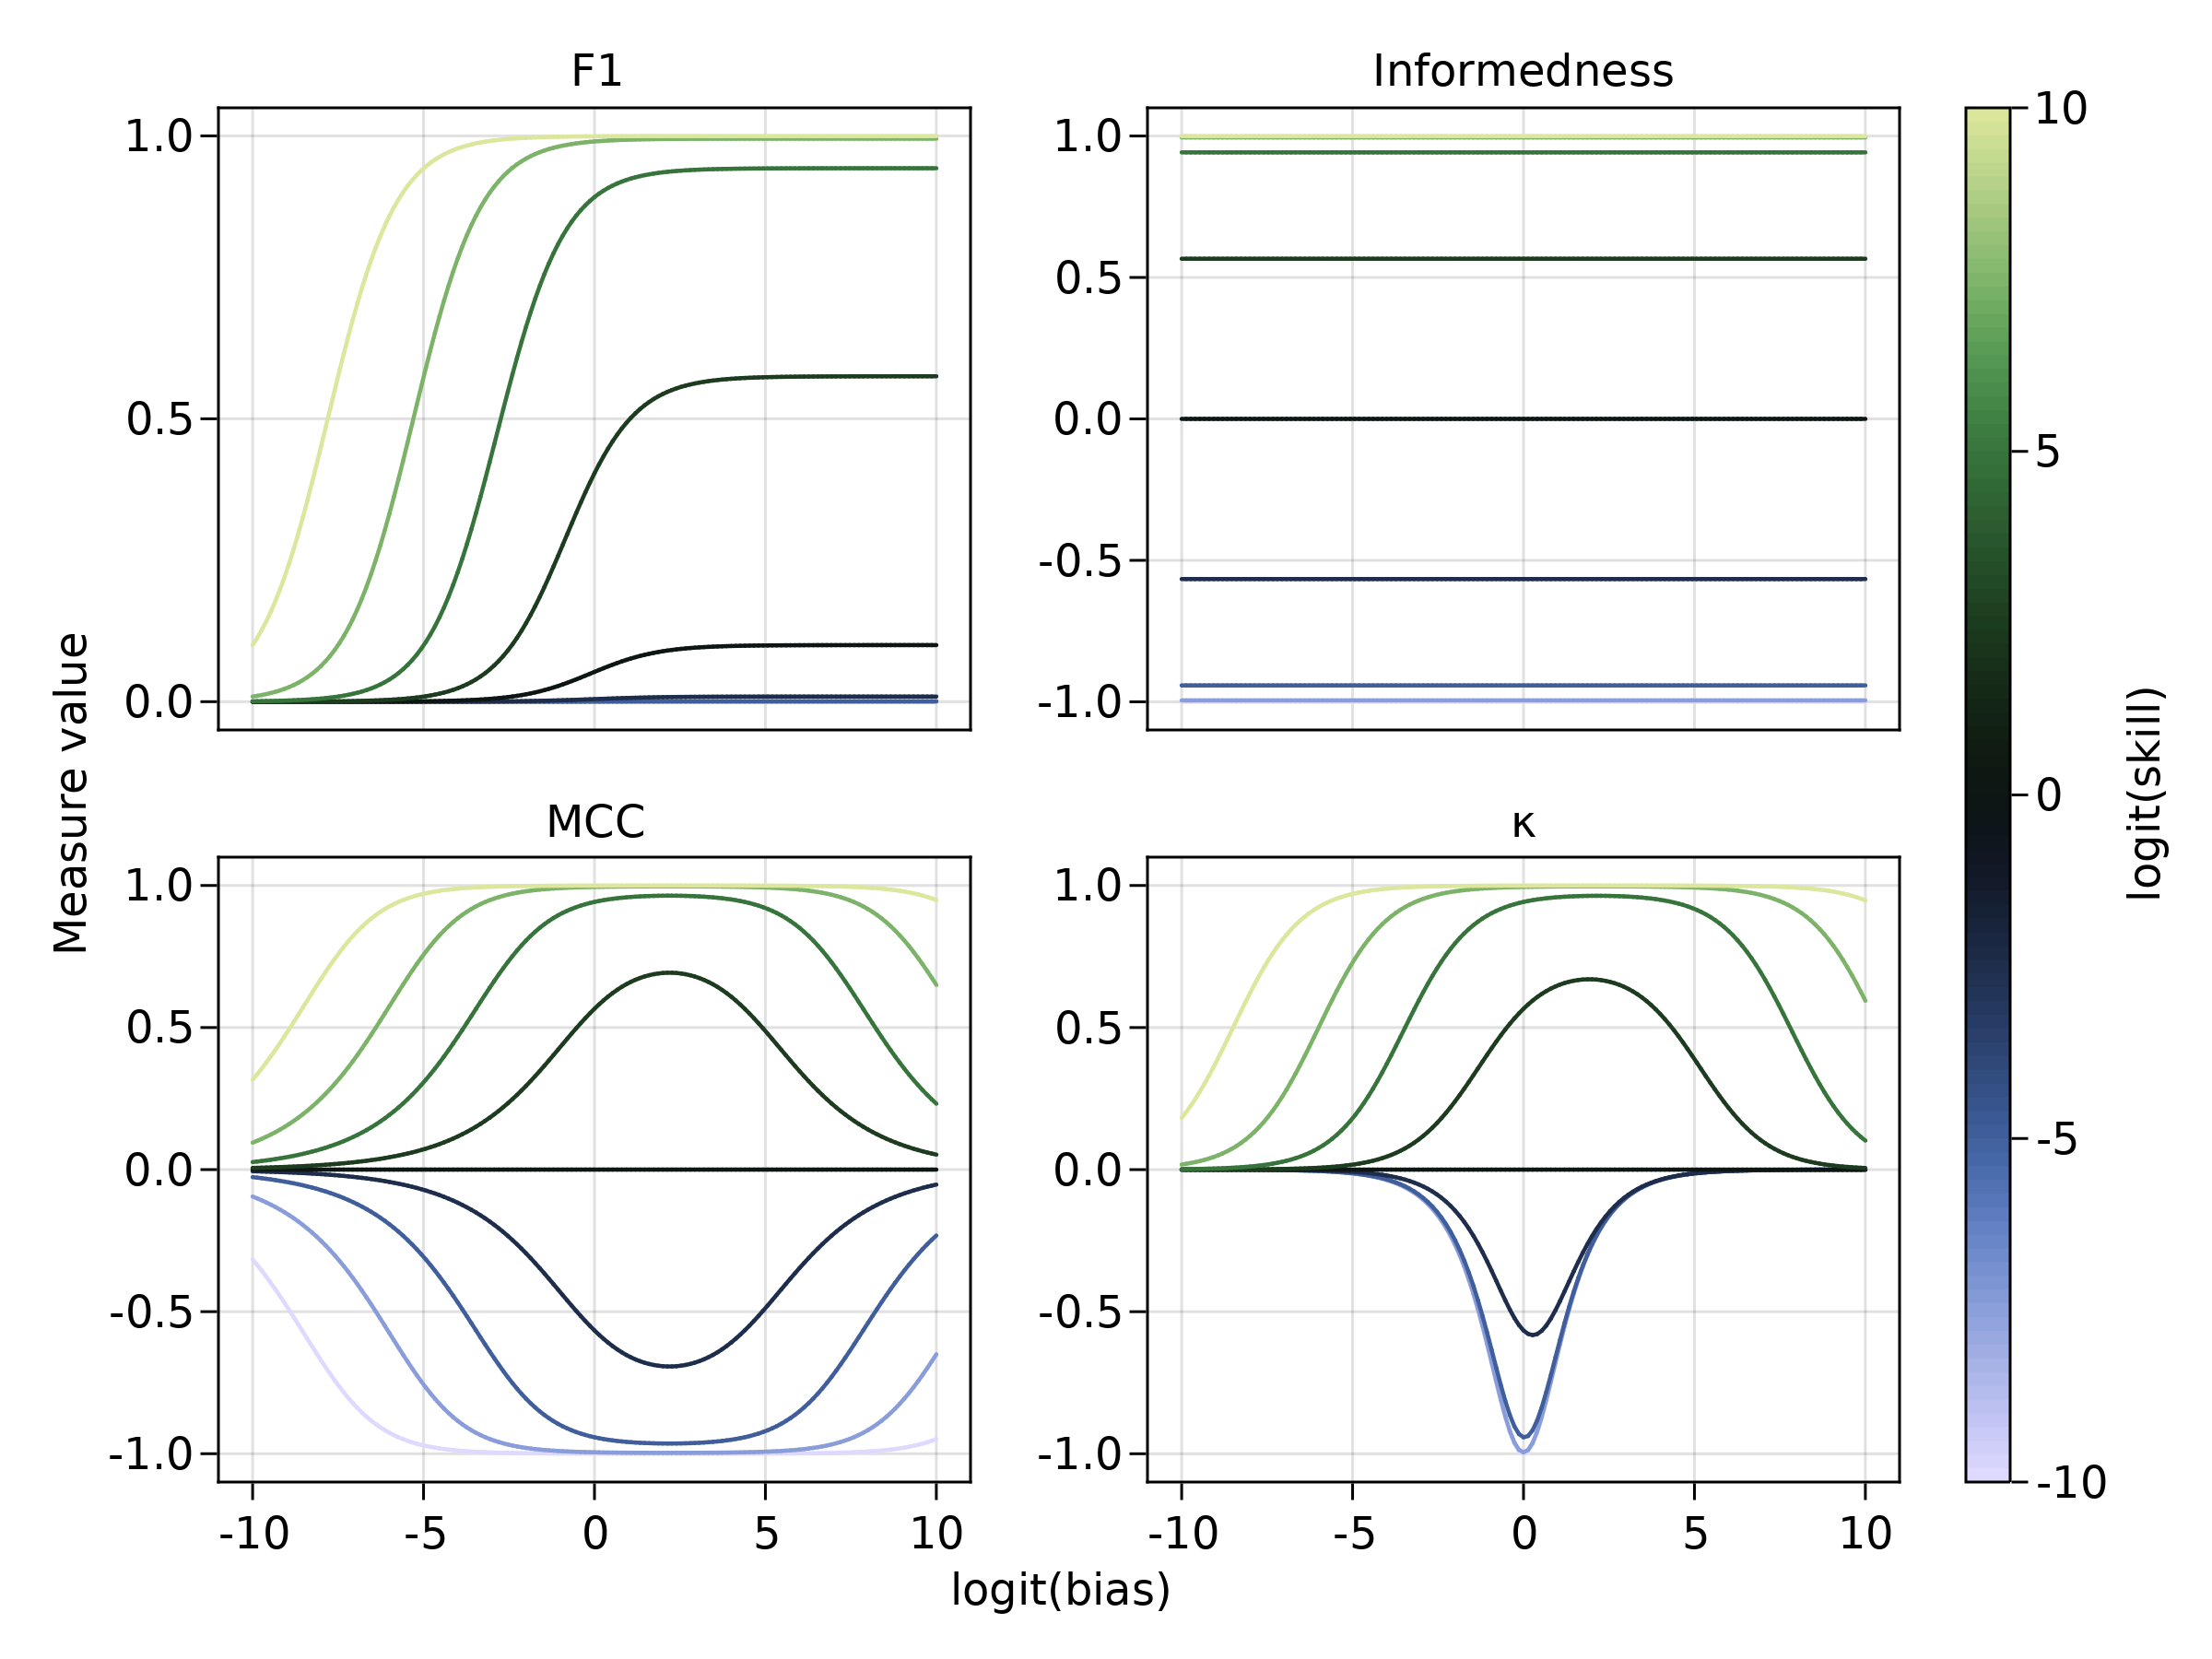
\includegraphics{figures/changing-bias.png}
\caption{Consequences of changing the classifier skills (\(s\)) and bias
(\(s\)) for a connectance \(\rho=0.15\), on accuracy, \(F_1\), postive
predictive value, and \(\kappa\). Accuracy increases with skill, but
also increases when the bias tends towards estimating \emph{fewer}
interactions. The \(F_1\) score increases with skill but also increases
when the bias tends towards estimating \emph{more} interactions; PPV
behaves in the same way. Interestingly, \(\kappa\) responds as expected
to skill (being negative whenever \(s < 0.5\)), and peaks for values of
\(b \approx 0.5\); nevertheless, the value of bias for which \(\kappa\)
is maximized in \emph{not} \(b=0.5\), but instead increases with
classifier skill. In other words, at equal skill, maximizing \(\kappa\)
would lead to select a \emph{more} biased classifier.}\label{fig:bias}
}
\end{figure}

In fig.~\ref{fig:bias}, we show that none of the four measures satisfy
all the considerations at once: \(F_1\) increases with skill, and
increases monotonously with bias; this is because \(F_1\) does not
account for true negatives, and the increase in positive detection masks
the over-prediction of interactions. Informedness varies with skill,
reaching 0 for a no-skill classifier, but is entirely unsensitive to
bias. Both MCC and \(\kappa\) have the same behavior, whereby they
increase with skill. \(\kappa\) peaks at increasing values of biass for
increasing skill, \emph{i.e.} is likely to lead to the selection of a
classifier that over-predicts interactions. By contract, MCC peaks at
the same value, regardless of skill, but this value is not
\(\text{logit}(b)=0\): unless at very high classifier skill, MCC risks
leading to a model that over-predicts interactions. In
fig.~\ref{fig:connectance}, we show that all measures except \(F_1\)
give a value of 0 for a no-skill classifier, and are forced towars their
correct maximal value when skill changes (\emph{i.e.} a more connected
networks will have higher values for a skilled classifierd, and lower
values for a classifier making mostly mistakes).

\begin{figure}
\hypertarget{fig:connectance}{%
\centering
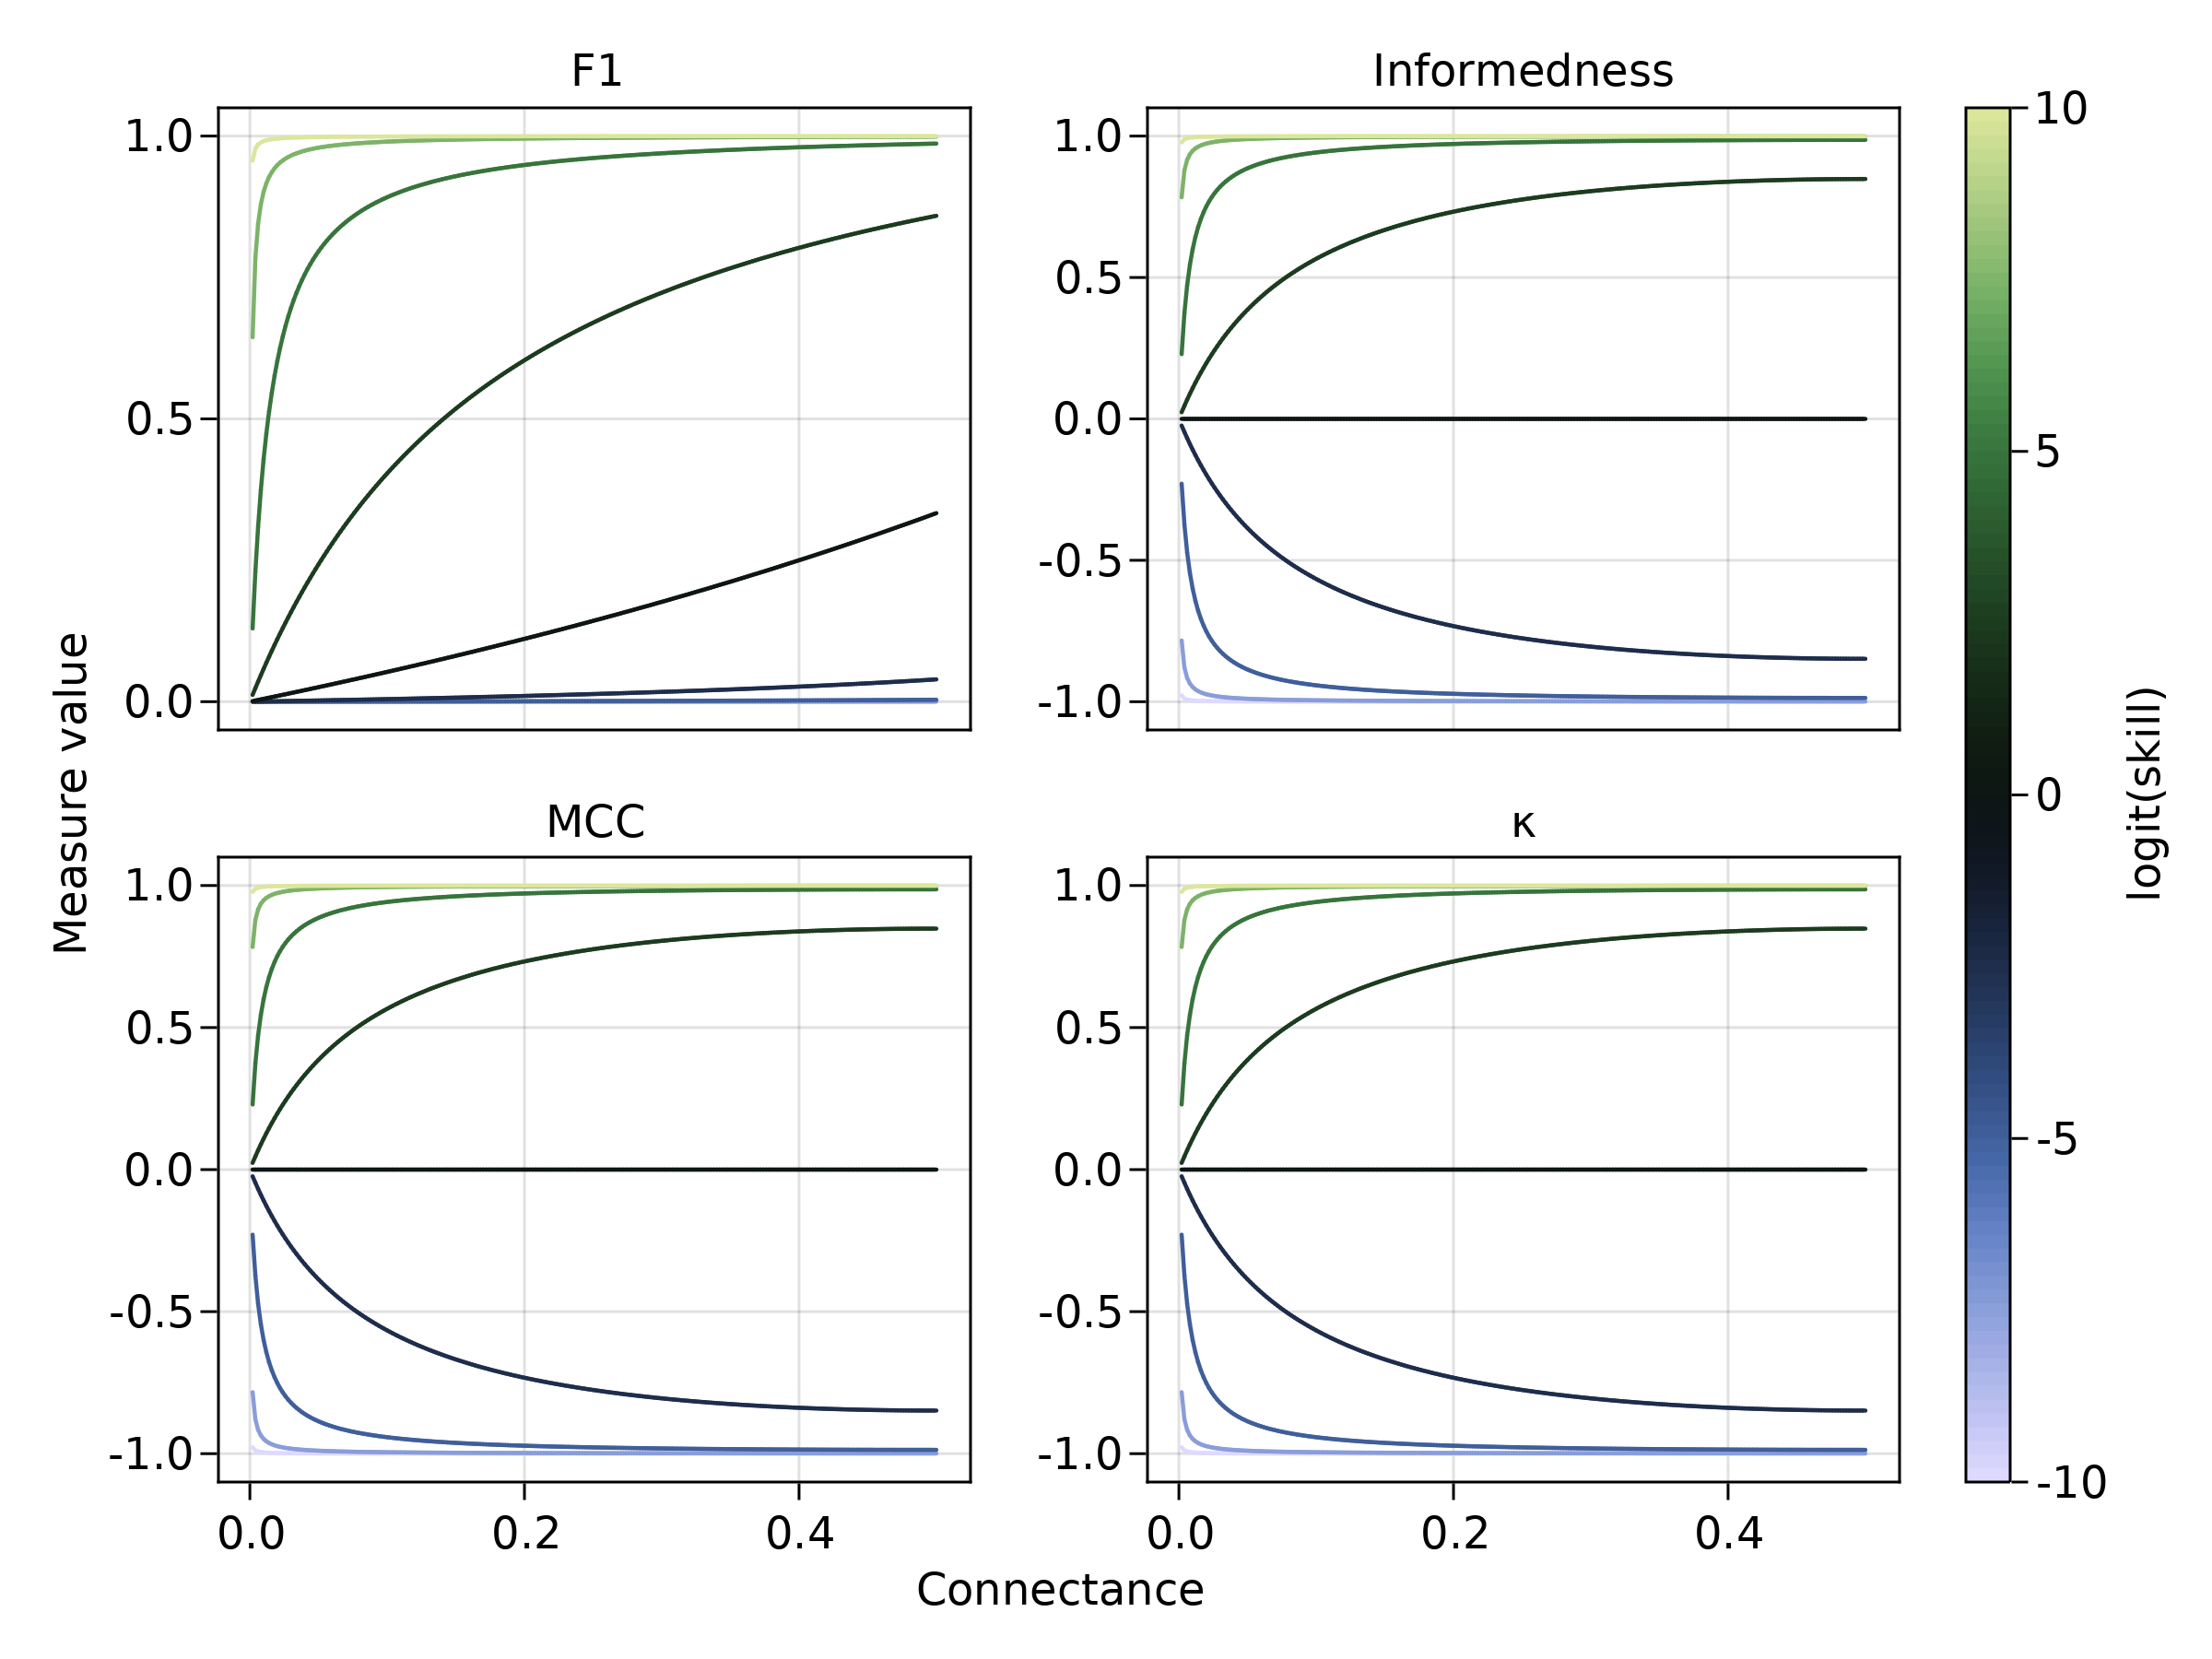
\includegraphics{figures/changing-connectance.png}
\caption{TODO}\label{fig:connectance}
}
\end{figure}

These two analyses point to the following recommendations: MCC is indeed
more appropriate than \(\kappa\), as although sensitive to bias, it is
sensitive in a consistent way. Informedness is appropriate at
discriminating between different skills, but confounded by bias. \(F_1\)
is increasing with bias, and should not be prioritized to evalue the
performance of the model. The discussion of sensitivity to bias should
come with a domain-specific caveat: although it is likely that
interactions documented in ecological networks are correct, a lot of
non-interactions are simply unobserved; as predictive models are used
for data-inflation (\emph{i.e.} the prediction of new interactions), it
is not necessarilly a bad thing to select models that predict more
interactions than the original dataset, because the original dataset
misses some interactions.

\hypertarget{illustration-on-empirical-food-webs}{%
\section{Illustration on empirical food
webs}\label{illustration-on-empirical-food-webs}}

In this section, we use a collection of XX empirical networks

\hypertarget{using-t-sbn-and-rdpg-to-simulate-arbitrarily-imperfect-classifier}{%
\subsection{Using t-SBN and RDPG to simulate arbitrarily imperfect
classifier}\label{using-t-sbn-and-rdpg-to-simulate-arbitrarily-imperfect-classifier}}

use t-SVD to only use some information

cumulative eigenvalues up to rank n give amount of information recovered

can be thresholded

how do values react to using fewer ranks

\hypertarget{effect-of-classifier-performance-on-metrics}{%
\subsection{Effect of classifier performance on
metrics}\label{effect-of-classifier-performance-on-metrics}}

\ldots{}

\hypertarget{numerical-experiments}{%
\section{Numerical experiments}\label{numerical-experiments}}

In the following section, we will generate random networks, and train
four binary classifiers (as well as an ensemble model using the sum of
the outputs) on 30\% of the interaction data. Networks are generated by
picking random generality \(g\) and vulnerability \(v\) traits for
\(S = 200\) species uniformly on the unit interval, and assigning an
interaction from species \(i\) to species \(j\) if
\(0.2g_i-\xi \le v_j \le 0.2g_i+\xi\), where \(\xi\) is a constant
regulating the connectance of the networks, and varies uniformly in
\([5\times 10^{-3}, 10^{-1}]\). This model gives fully interval networks
that are close analogues to the niche model (Williams \& Martinez,
2000), but has the benefit of only relying on two features
(\(g_i, v_j\)), and having the exact same rule for all interactions. It
is, therefore, a simple case which most classifiers should be able to
learn.

The training sample is composed of 30\% of the \(4\times 10^4\) possible
entries in the network, \emph{i.e.} \(n=12000\). Out of these
interactions, we pick a proportion \(\nu\) (the training set bias) to be
positive, so that the training set has \(\nu n\) interactions, and
\((1-\nu) n\) non-interactions. We vary \(\nu\) uniformly in \(]0,1[\).
This allows to evaluate how the measures of binary classification
performance respond to artificially rebalanced dataset for a given
network connectance. Note that both \(\xi\) and \(\nu\) are sampled from
a distribution rather than being picked on a grid; this is because there
is no direct relationship between the value of \(\xi\) and the
connectance of the simulated network, and therefore the precise value of
\(\xi\) is not relevant for the analysis of the results.

The dataset used for numerical experiments is composed of 64000 such
\((\xi, \nu)\) pairs, on which four learners are trained: a decision
tree regressor, a boosted regression tree, a ridge regressor, and a
random forest regressor. All models were taken from the \texttt{MLJ.jl}
package (Blaom et al., 2020; Blaom \& Vollmer, 2020) in Julia 1.7
(Bezanson et al., 2017). In order to pick the best adjacency matrix for
a given learner, we performed a thresholding approach using 500 steps on
predictions from the testing set, and picking the threshold that
maximized Youden's informedness, which is usually the optimized target
for imbalanced classification. During the thresholding step, we measured
the area under the receiving-operator characteristic (ROC-AUC) and
precision-recall (PR-AUC) curves, as measures of overall performance
over the range of returned values. We report the ROC-AUC and PR-AUC, as
well as a suite of other measures as introduced in the next section, for
the best threshold. The ensemble model was generated by summing the
predictions of all component models on the testing set (ranged in
\([0,1]\)), then put through the same thresholding process. The complete
code to run the simulations is given as an appendix; running the final
simulation required 4.8 core days (approx. 117 hours).

After the simulations were completed, we removed all runs (\emph{i.e.}
pairs of \(\xi\) and \(\nu\)) for which at least one of the following
conditions was met: the accuracy was 0, the true positive or true
negative rates were 0, the connectance was larger than 0.2. This removes
both the obviously failed model runs, and the networks that are more
densely connected compared to the connectance of empirical food webs
(and are therefore less difficult to predict, being less imbalanced).

\hypertarget{effect-of-training-set-bias-on-performance}{%
\subsection{Effect of training set bias on
performance}\label{effect-of-training-set-bias-on-performance}}

In fig.~\ref{fig:biasmccinf}, we present the response of MCC and
informedness to (i) four levels of network connectance and (ii) a
gradient of training set bias, for the four component models as well as
the ensemble. All models reached a higher performance on more connected
networks, and using more biased training sets (with the exception of
ridge regression, whose informedness decreased in performance with
training set bias). In all cases, informedness was extremely high, which
is an expected consequence of the fact that this is the value we
optimized to determine the cutoff. MCC increased with training set bias,
although this increase became less steep with increasing connectance.
Interestingly, the ensemble almost always outclassed its component
models.

\begin{figure}
\hypertarget{fig:biasmccinf}{%
\centering
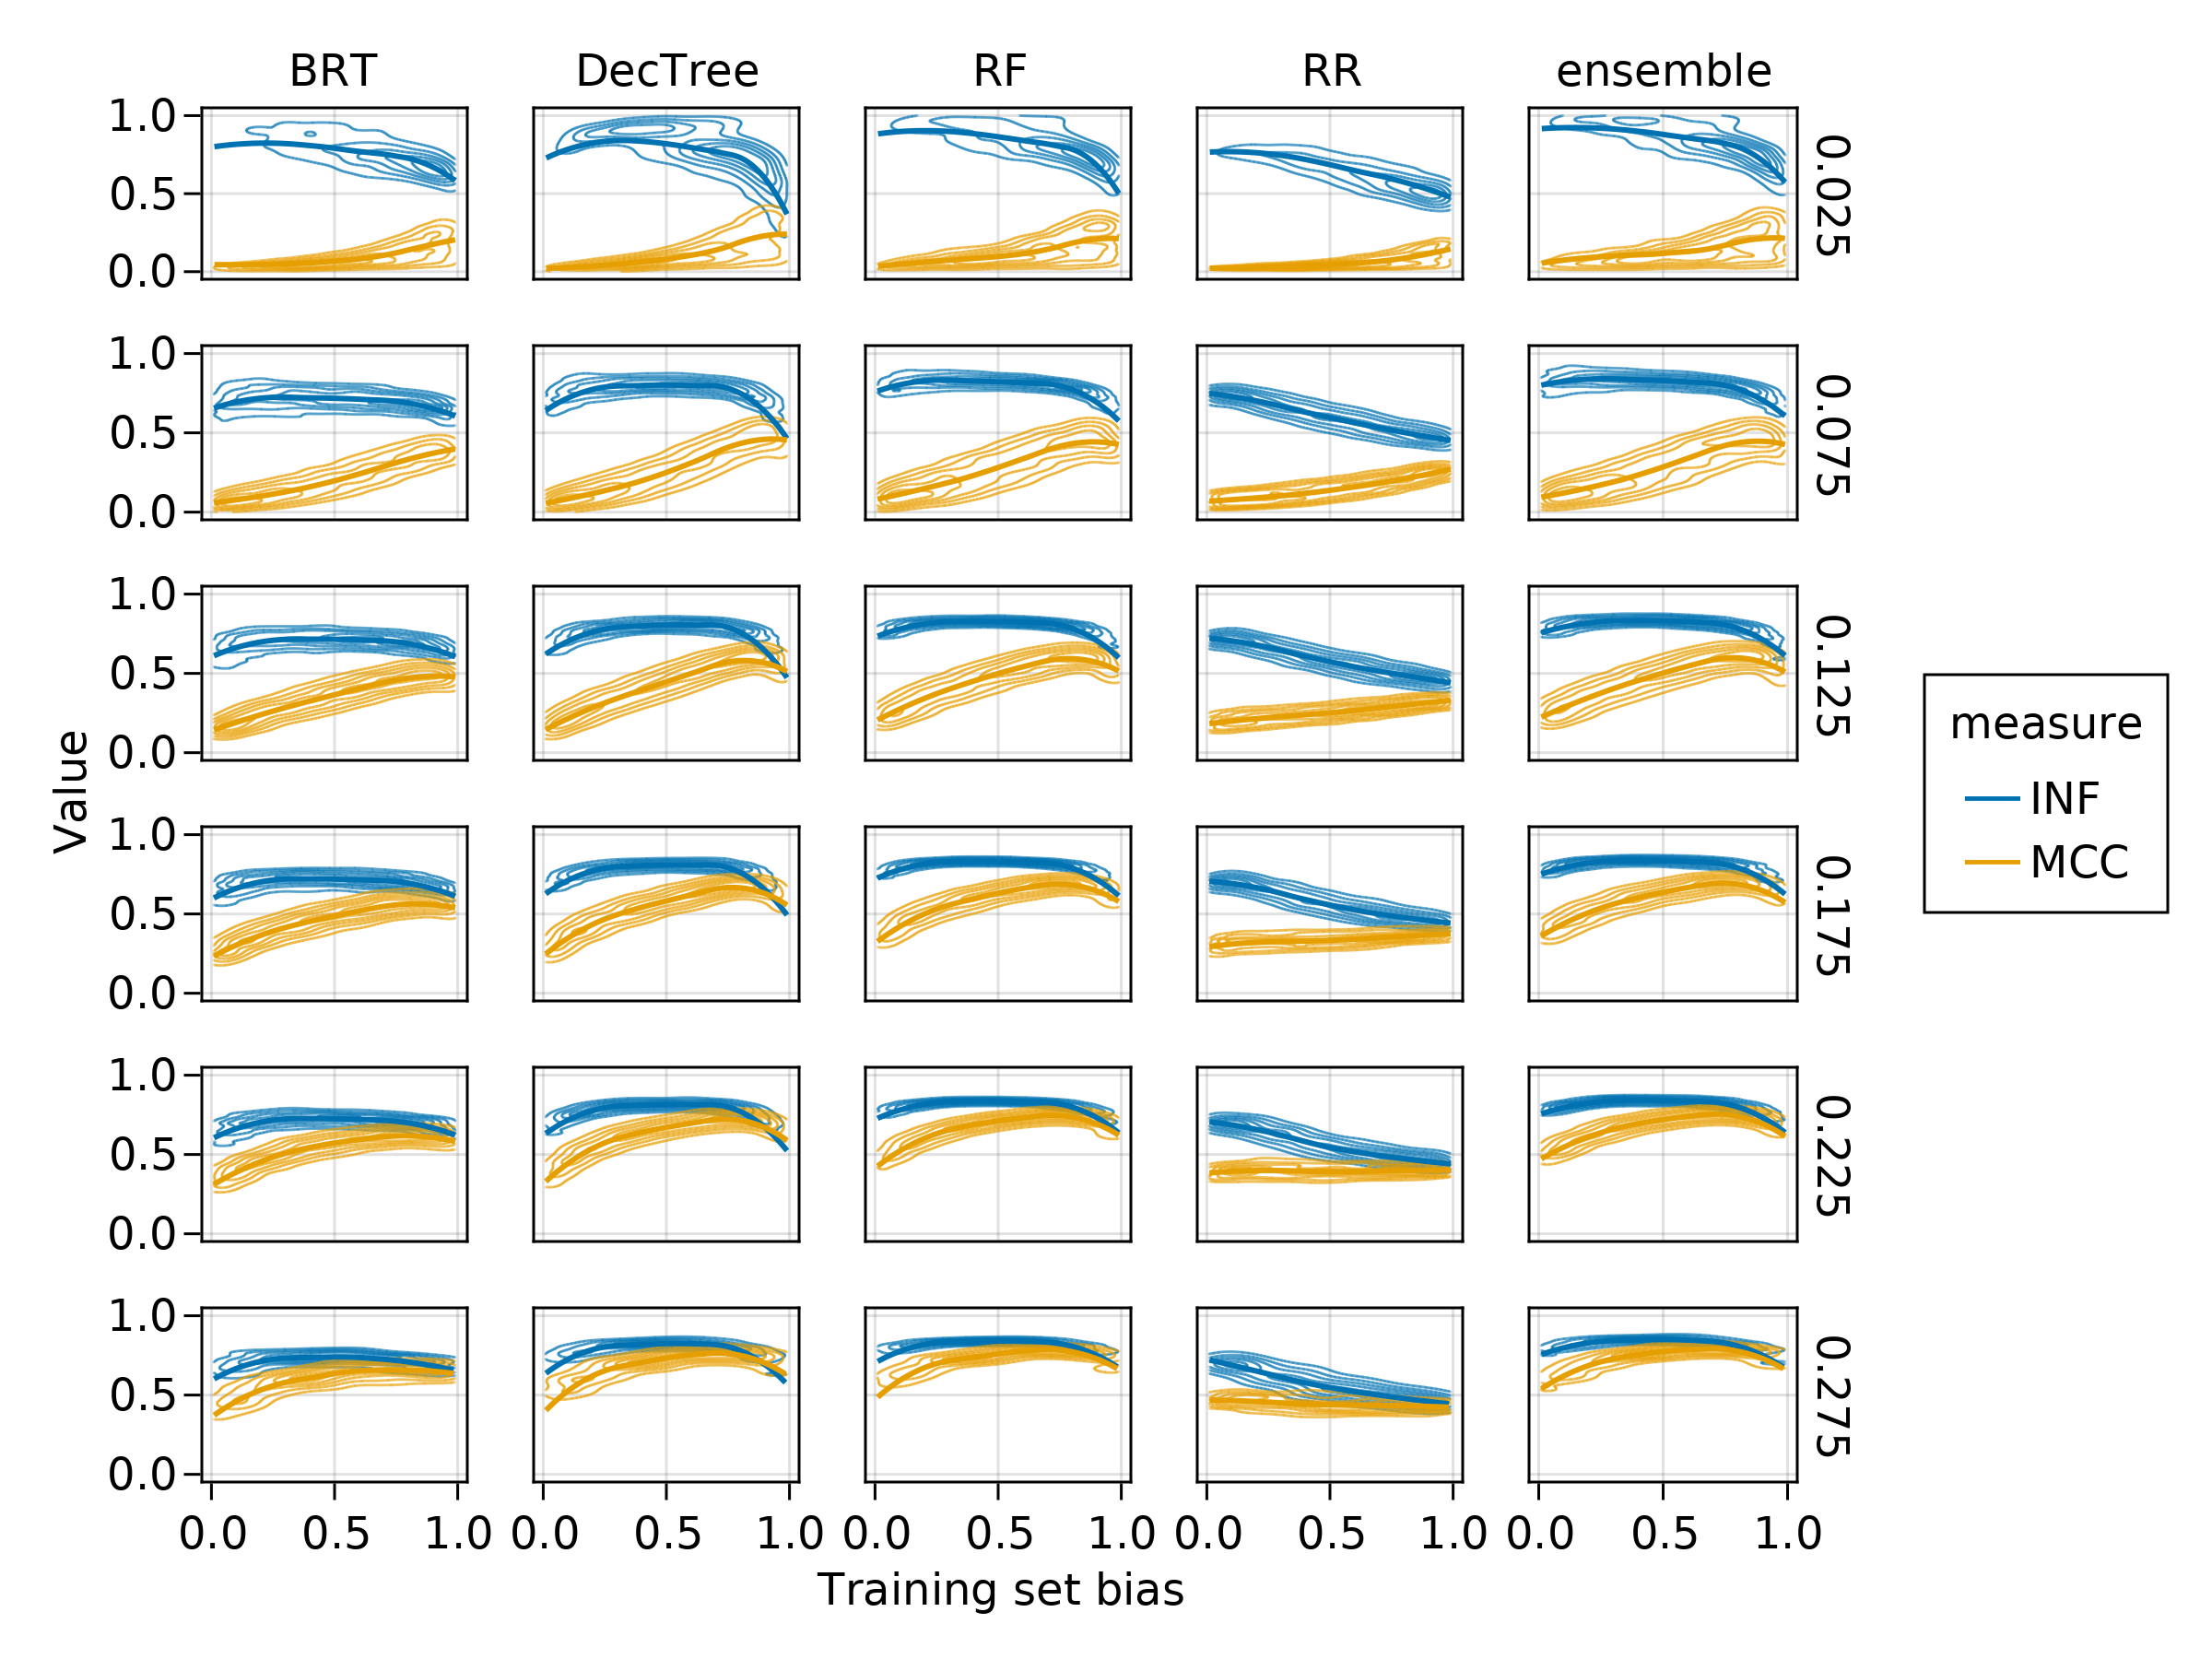
\includegraphics{figures/bias_mcc_inf.png}
\caption{TODO}\label{fig:biasmccinf}
}
\end{figure}

In fig.~\ref{fig:biasrocpr}, we present the same information as
fig.~\ref{fig:biasmccinf}, this time using ROC-AUC and PR-AUC. ROC-AUC
is always high, and does not vary with training set bias. On the other
hand, PR-AUC shows very strong responses, increasing with training set
bias. It is notable here that two classifiers that seemed to be
performing well (Decision Tree and Random Forest) based on their MCC are
not able to reach a high PR-AUC even at higher connectances. As in
fig.~\ref{fig:biasmccinf}, the ensemble outperforms its component
models.

\begin{figure}
\hypertarget{fig:biasrocpr}{%
\centering
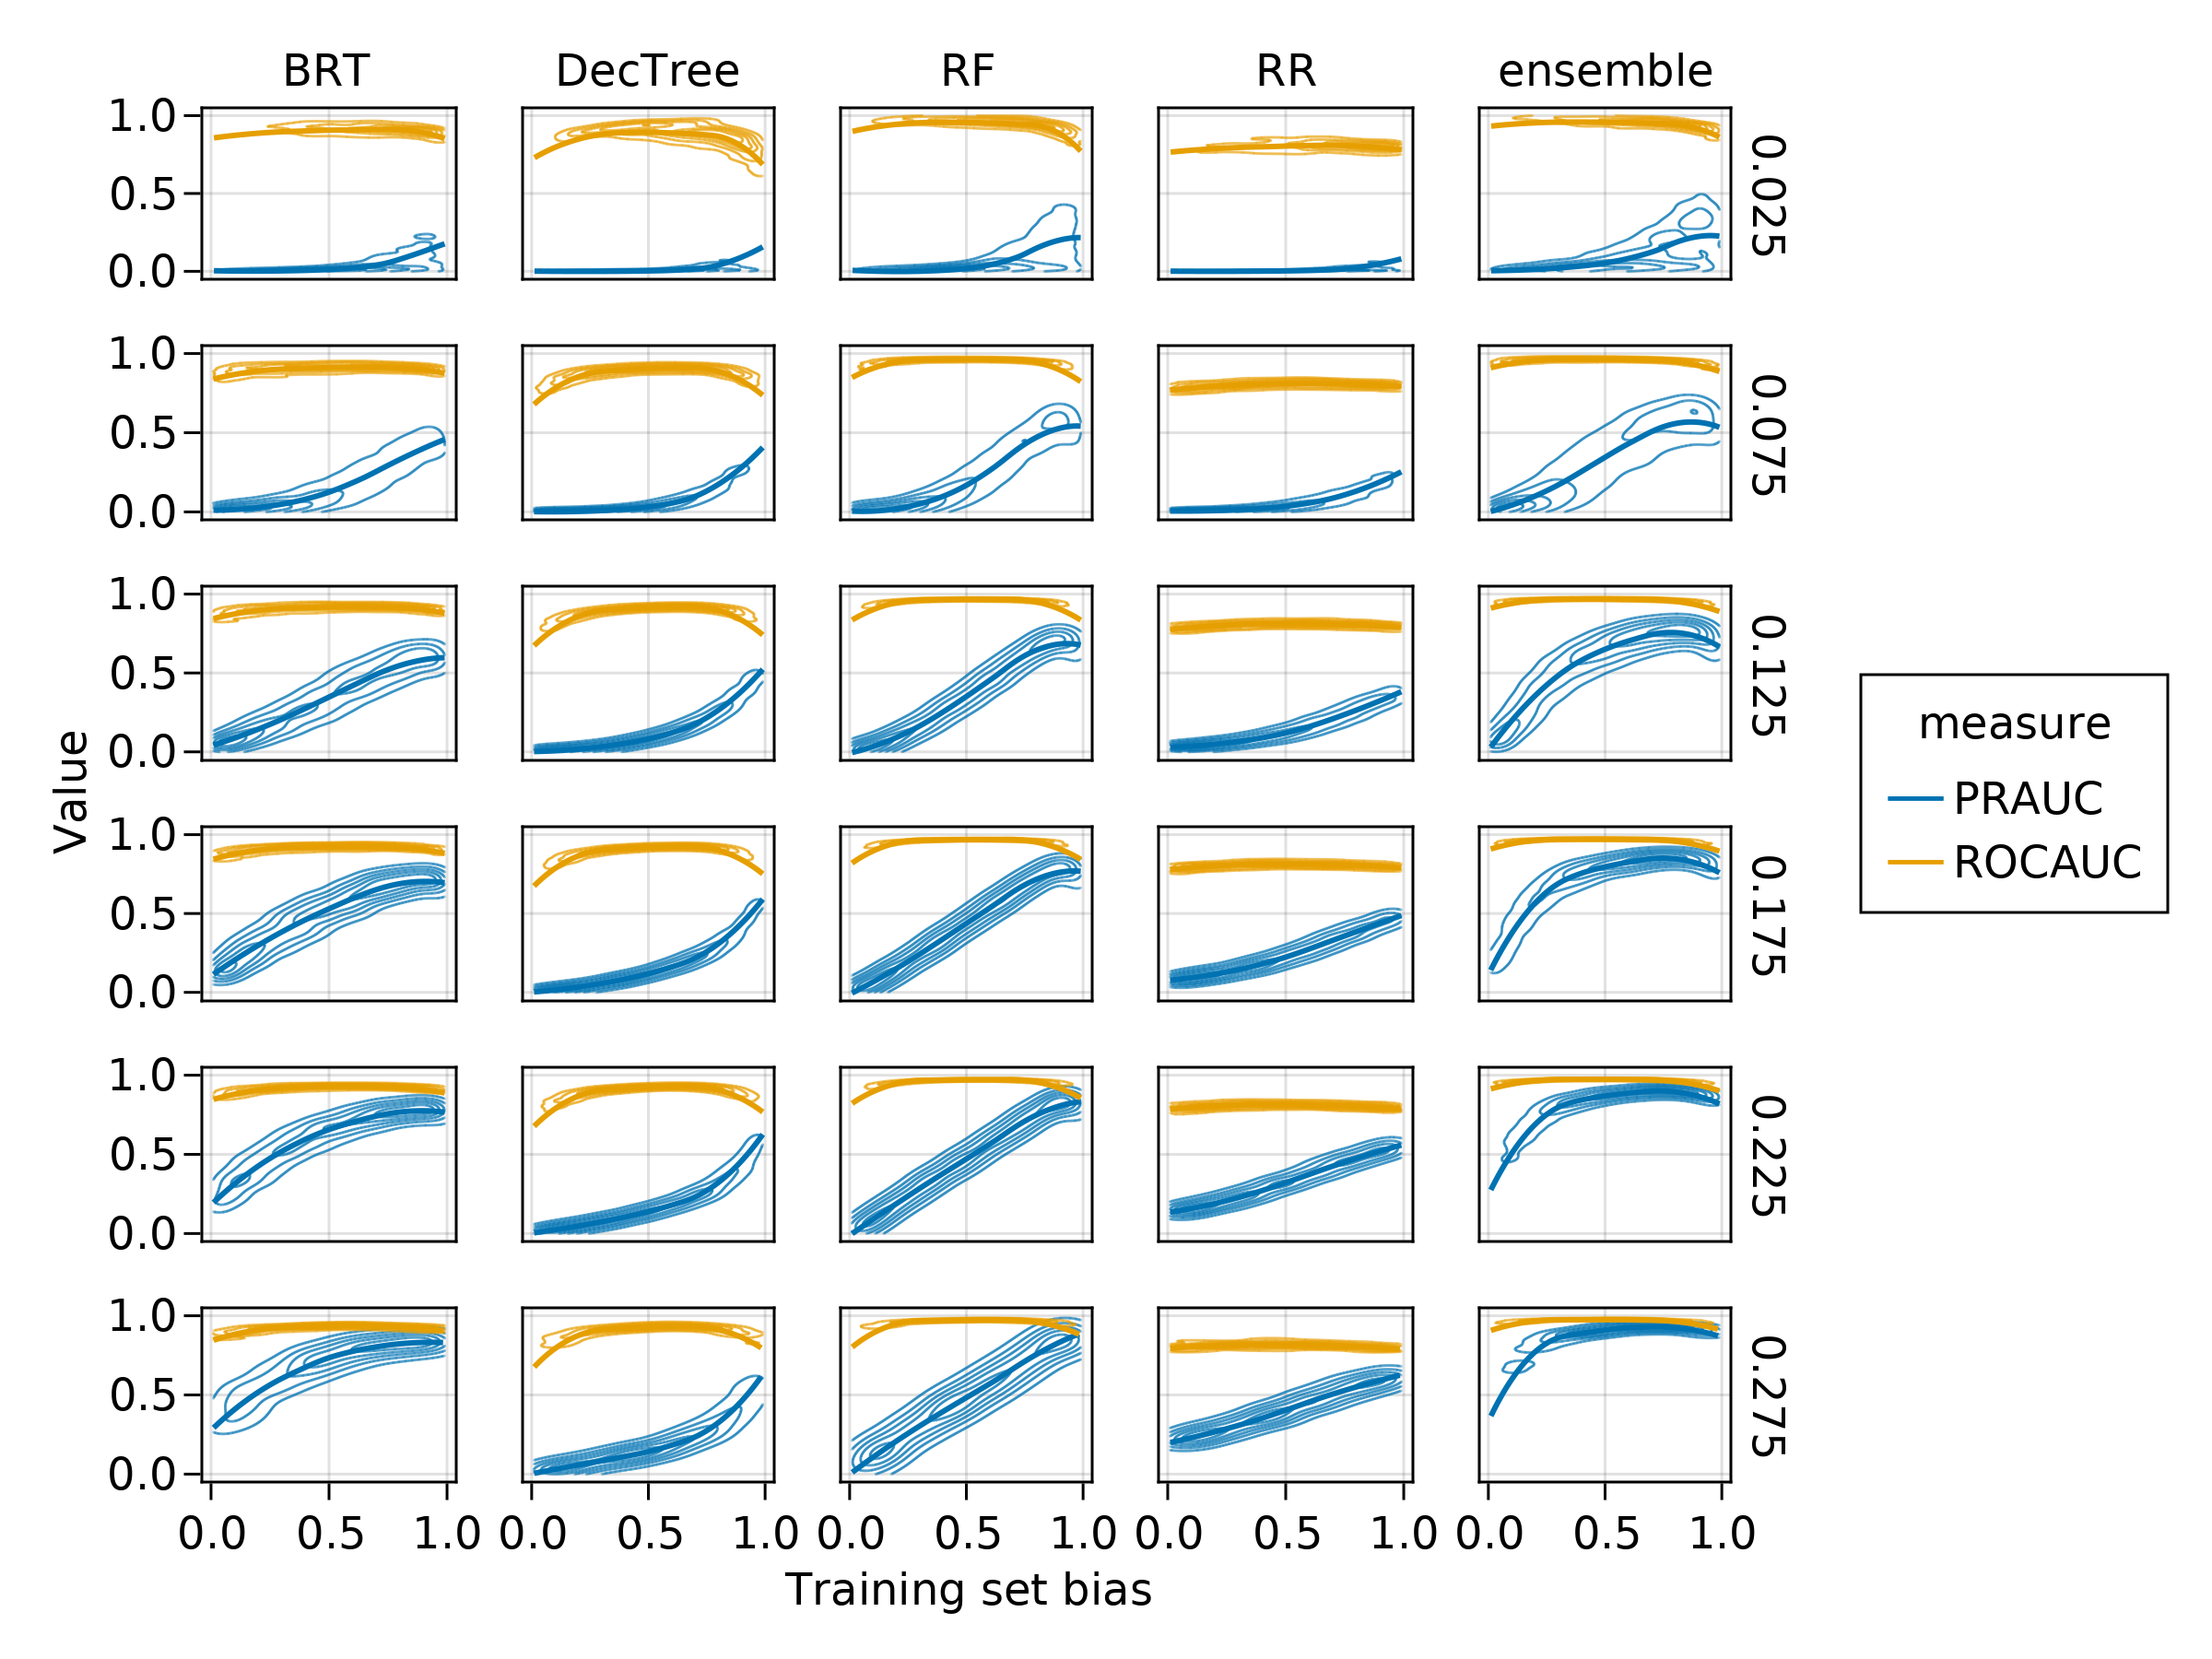
\includegraphics{figures/bias_roc_pr.png}
\caption{TODO}\label{fig:biasrocpr}
}
\end{figure}

Based on the results presented in fig.~\ref{fig:biasmccinf} and
fig.~\ref{fig:biasrocpr}, it seems that informedness and ROC-AUC are not
necessarilly able to discriminate between good and bad classifiers
(although this result may be an artifact for informedness, as it has
been optimized when thresholding). On the other hand, MCC and PR-AUC
show a strong response to training set bias, and may therefore be more
useful at model comparison.

\hypertarget{required-amount-of-positives-to-get-the-best-performance}{%
\subsection{Required amount of positives to get the best
performance}\label{required-amount-of-positives-to-get-the-best-performance}}

The previous results revealed that the measure of classification
performance responds both to the bias in the training set \emph{and} to
the connectance of the network; from a practical point of view,
assembling a training set requires to withold positive information,
which in ecological networks are very scarce (and typically more
valuable than negatives, on which there is a doubt). For this reason,
across all values of connectance, we measured the training set bias that
maximized a series of performance measures. When this value is high, the
training set needs to skew positive in order to get a good model; when
this value is about 0.5, the training set needs to be artificially
balanced to optimize the model performance. These results are presented
in fig.~\ref{fig:optimbias}.

\begin{figure}
\hypertarget{fig:optimbias}{%
\centering
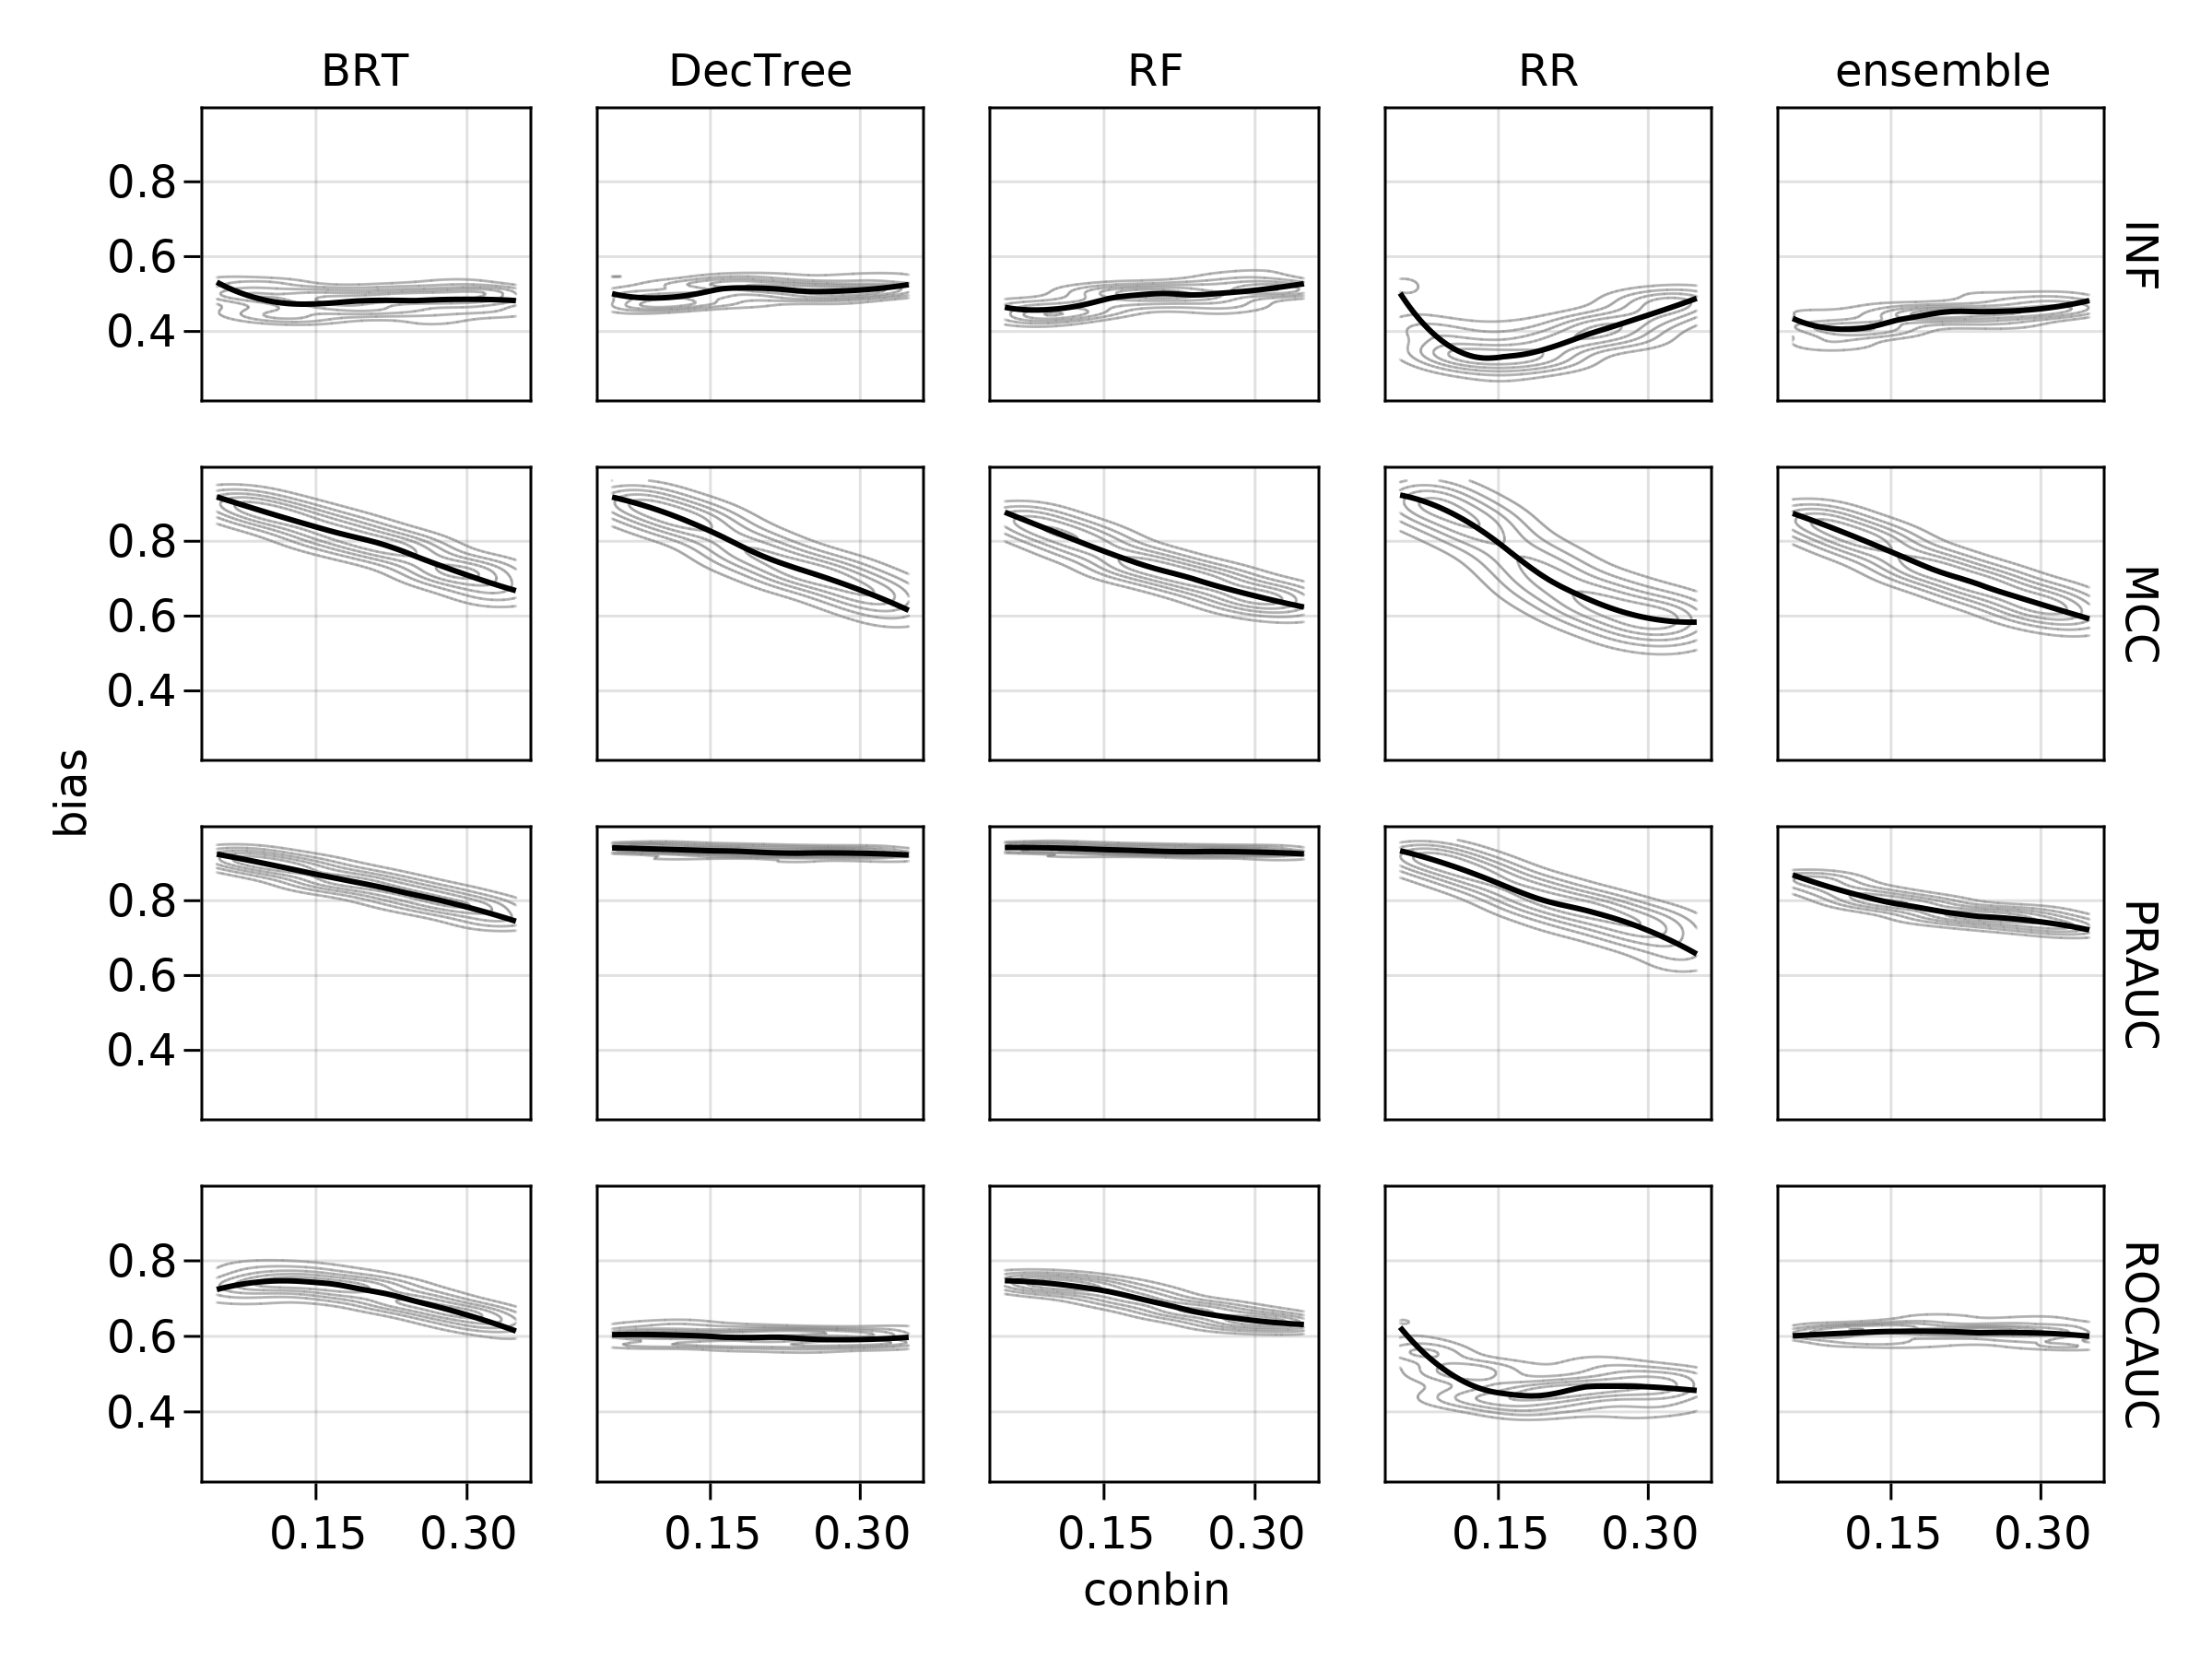
\includegraphics{figures/optim_bias.png}
\caption{TODO}\label{fig:optimbias}
}
\end{figure}

Interestingly, as long as the connectance of the network was above
\(\approx 0.1\), the optimal prevalence in the training set is 0.5,
\emph{i.e.} as many positives as negatives. Low connectance is usually
achieved for very large networks, due to the scaling relationship
between richness and links (MacDonald et al., 2020). Therefore, larger
networks may require \emph{more} biasing of the training set in order to
be optimally predicted, whereas smaller, more connected networks may
not. It is worth noting that the optimal bias for the training set
stabilizes at 0.5 regardless of connectance \emph{and} model \emph{and}
measure of model evaluation.

\begin{figure}
\hypertarget{fig:optimperf}{%
\centering
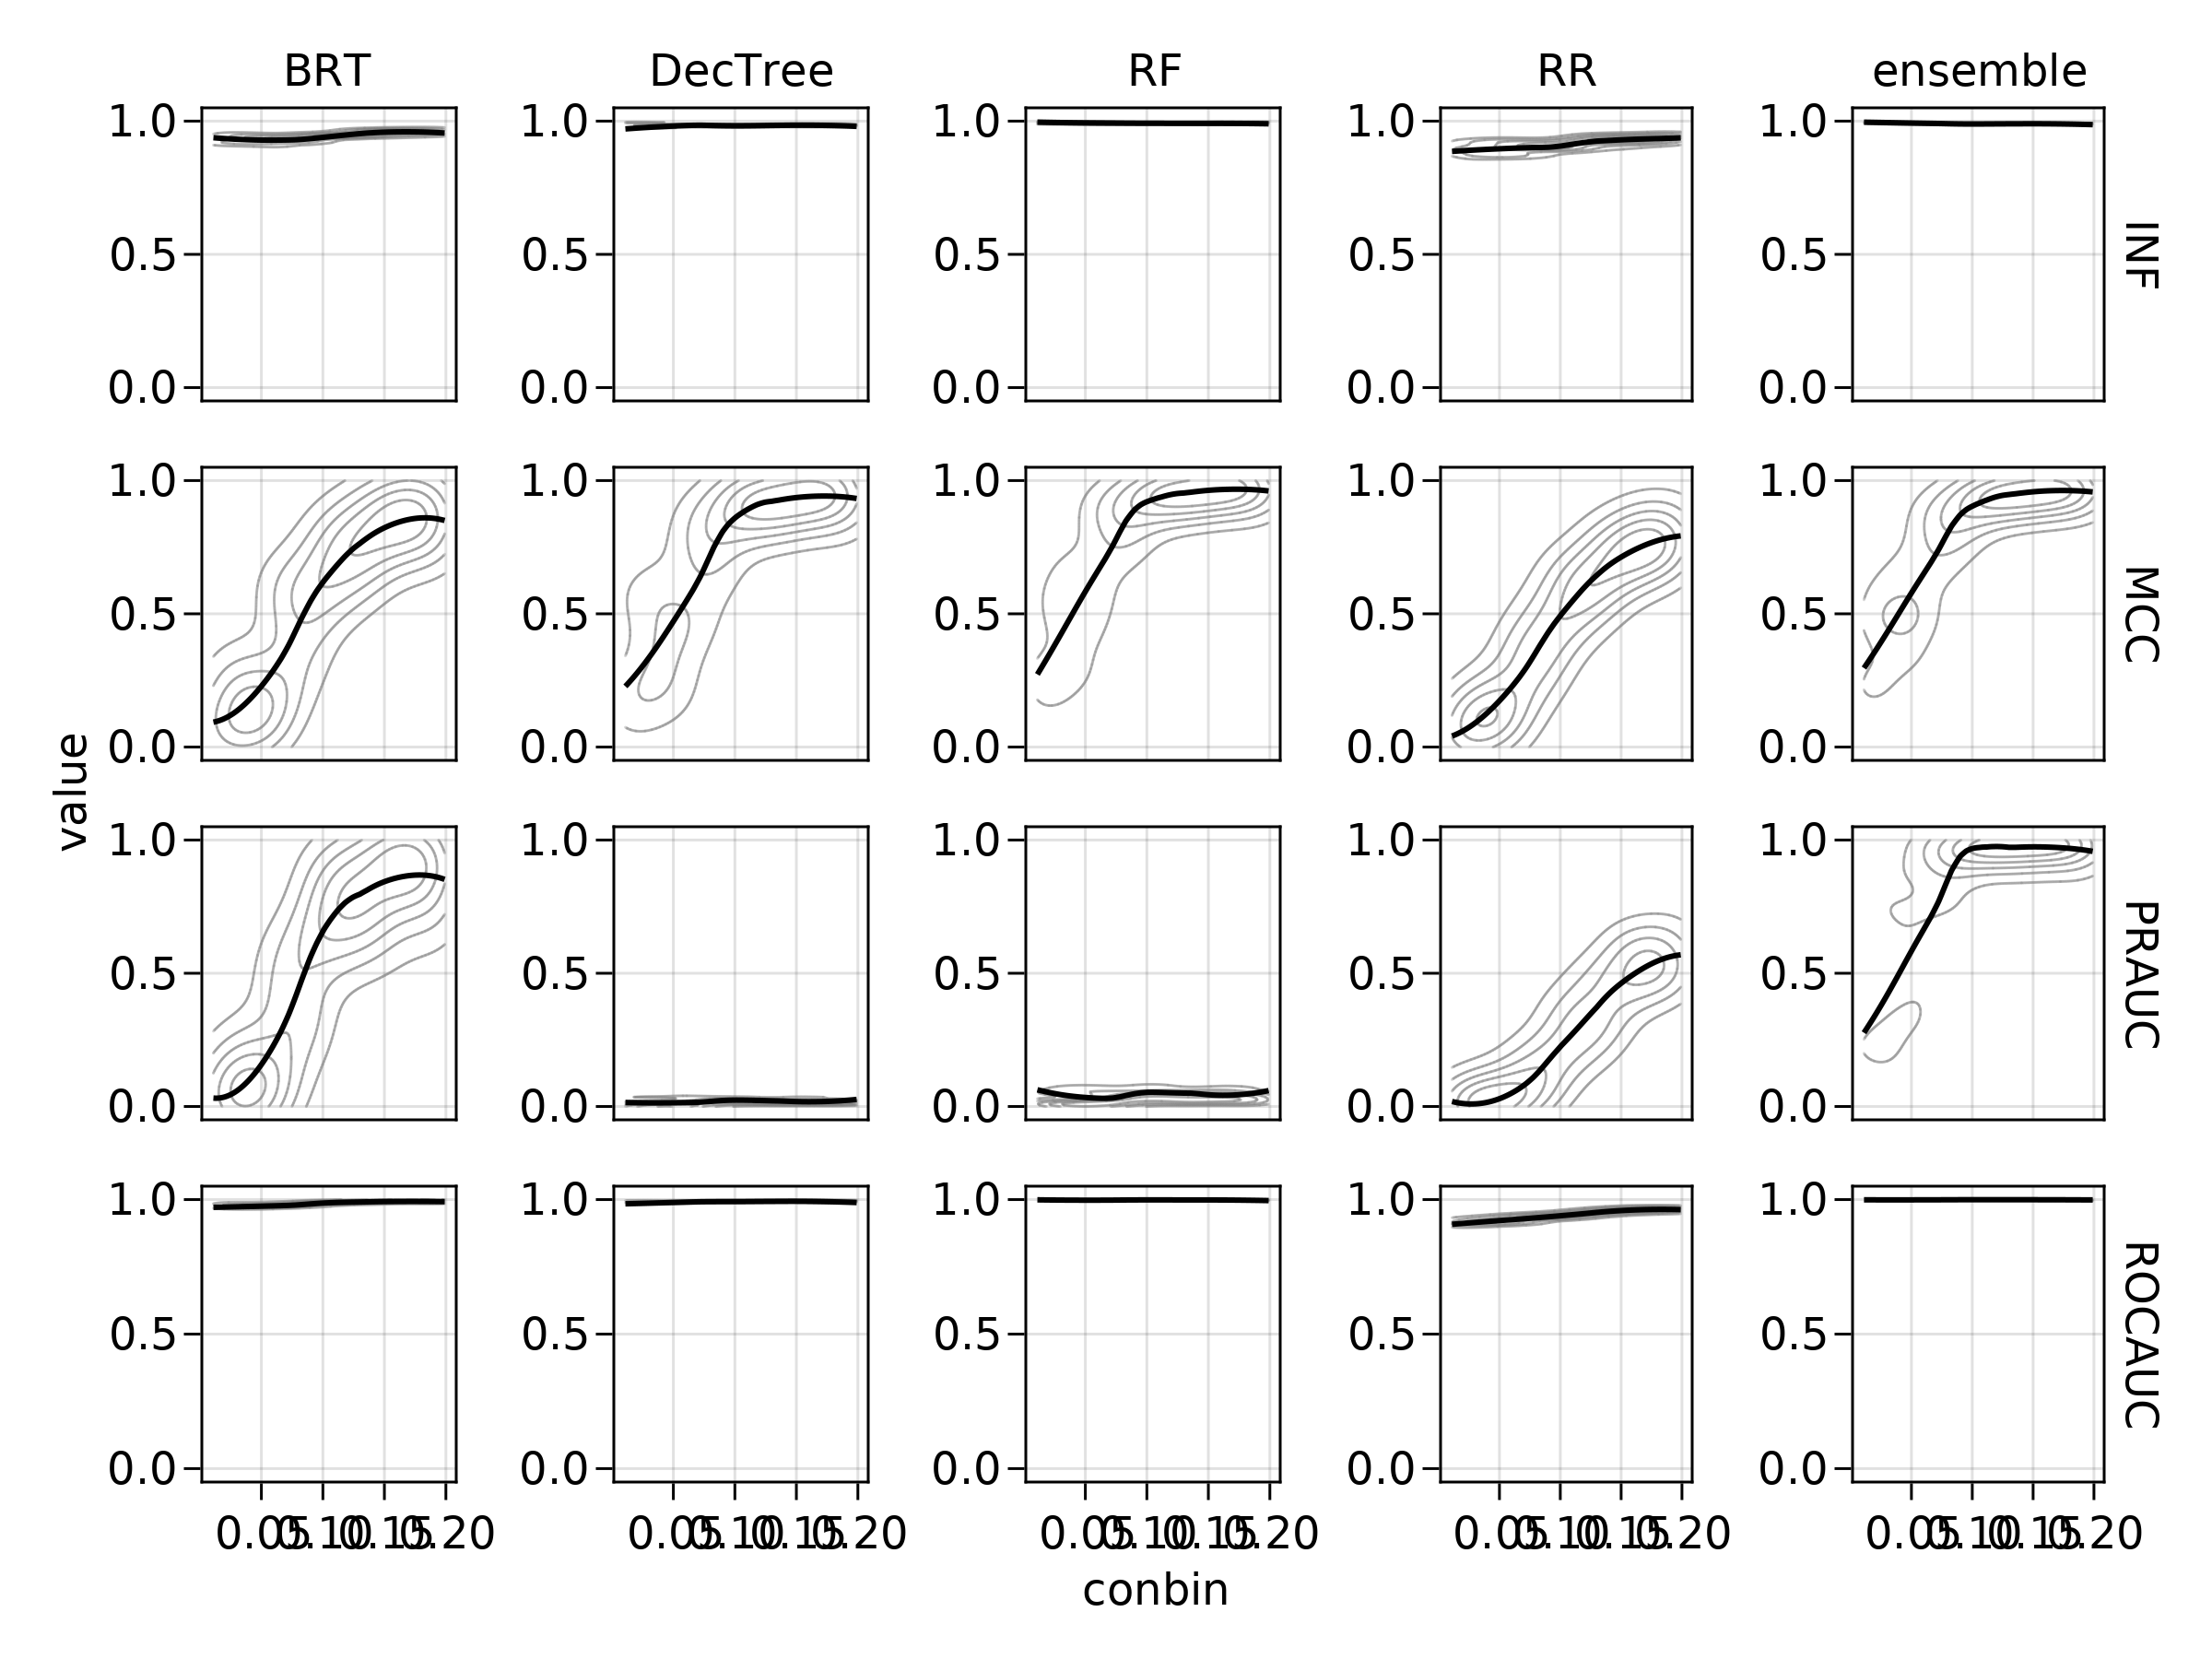
\includegraphics{figures/optim_perf.png}
\caption{TODO}\label{fig:optimperf}
}
\end{figure}

\hypertarget{guidelines-for-the-assesment-of-network-predictive-models}{%
\section{Guidelines for the assesment of network predictive
models}\label{guidelines-for-the-assesment-of-network-predictive-models}}

The results presented here highlight an interesting paradox: larger
networks (with lower connectance) require more training set bias in
order to maximize model performance fig.~\ref{fig:optimbias}, but are
also more difficult to predict according to MCC and PR-AUC
fig.~\ref{fig:optimperf}. This suggests that the task of network
prediction will be difficult regardless of network size: by being
limited by the \emph{frequency} of interactions when the network is
large, and by being limited by the \emph{number} of interactions when
the network is small. Nevertheless, based on the simulations and
numerical experiments, it is possible to formulate a series of
recommendations for the evaluation of network prediction models.

First, because we should have more trust in reported interactions than
in reported absences of interactions, we can draw on previous literature
to recommend informedness as a measure to decide on a threshold (Chicco
et al., 2021); this being said, because informedness is insensitive to
bias, the model performance is better evaluated through the use of MCC
fig.~\ref{fig:biasmccinf}. Because \(F_1\) is monotonously sensitive to
classifier bias fig.~\ref{fig:bias} and network connectance
fig.~\ref{fig:connectance}, MCC should be prefered as a measure of model
evaluation.

Second, because the PR-AUC responds more to network connectance
fig.~\ref{fig:optimperf} and training set imbalance
fig.~\ref{fig:biasrocpr}, it should be used as a measure of model
performance over the ROC-AUC. This is not to say that ROC-AUC should be
discarded (in fact, a low ROC-AUC is a sign of an issue with the model),
but that its interpretation should be guided by the PR-AUC value. This
again echoes recommendations from other fields (Saito \& Rehmsmeier,
2015).

Thirdly, regardless of network connectance \emph{or} measure to evaluate
the model performance, as long as the network connectance is larger than
\(\approx 0.1\), artificially balancing the training set to have
equiprevalence will give the best possible results. This was true for
all models.

Finally, it is noteworthy that the ensemble model was systematically
better than the component models; even when poor models were included
(Random Forest and Decision Tree), the ensemble was able to leverage the
different biases expressed by the models to make an overall more
accurate prediction. We do not expect that ensembles will \emph{always}
be better than single models. In a recent multi-model comparison, Becker
et al. (2021) found that the ensemble was \emph{not} the best model.
There is no general conclusion to draw from this besides reinforcing the
need to be pragmatic about which models should be included in the
ensemble, or whether to use an ensemble at all. In a sense, the
surprising peformance of the ensemble model should form the basis of the
last recommendation: optimal training set bias and its interaction with
connectance and binary classifier is, in a sense, an hyperparameter that
should be assessed. The distribution of results in
fig.~\ref{fig:optimbias} and fig.~\ref{fig:optimperf} show that there
are variations around the trend; furthermore, networks with different
structures than the one we simulated here may respond in different ways.

\textbf{Acknowledgements:} We acknowledge that this study was conducted
on land within the traditional unceded territory of the Saint Lawrence
Iroquoian, Anishinabewaki, Mohawk, Huron-Wendat, and Omàmiwininiwak
nations. This research was enabled in part by support provided by Calcul
Québec (www.calculquebec.ca) and Compute Canada (www.computecanada.ca)
through the Narval general purpose cluster. TP is supported by a NSERC
Discovery Grant and Discovery Acceleration Supplement, and by a grant
from the Institut de Valorisation des Données (IVADO).

\hypertarget{references}{%
\section*{References}\label{references}}
\addcontentsline{toc}{section}{References}

\hypertarget{refs}{}
\begin{CSLReferences}{1}{0}
\leavevmode\hypertarget{ref-Allouche2006AssAcc}{}%
Allouche, O., Tsoar, A., \& Kadmon, R. (2006). Assessing the accuracy of
species distribution models: Prevalence, kappa and the true skill
statistic (TSS). \emph{Journal of Applied Ecology}, \emph{43}(6),
1223--1232. \url{https://doi.org/10.1111/j.1365-2664.2006.01214.x}

\leavevmode\hypertarget{ref-Becker2021OptPre}{}%
Becker, D., Albery, G. F., Sjodin, A. R., Poisot, T., Bergner, L.,
Dallas, T., Eskew, E. A., Farrell, M. J., Guth, S., Han, B. A., Simmons,
N. B., Stock, M., Teeling, E. C., \& Carlson, C. J. (2021). Optimizing
predictive models to prioritize viral discovery in zoonotic reservoirs.
\emph{bioRxiv}, 2020.05.22.111344.
\url{https://doi.org/10.1101/2020.05.22.111344}

\leavevmode\hypertarget{ref-Bezanson2017JulFre}{}%
Bezanson, J., Edelman, A., Karpinski, S., \& Shah, V. (2017). Julia: A
Fresh Approach to Numerical Computing. \emph{SIAM Review}, \emph{59}(1),
65--98. \url{https://doi.org/10.1137/141000671}

\leavevmode\hypertarget{ref-Blaom2020MljJul}{}%
Blaom, A. D., Kiraly, F., Lienart, T., Simillides, Y., Arenas, D., \&
Vollmer, S. J. (2020). MLJ: A Julia package for composable machine
learning. \emph{Journal of Open Source Software}, \emph{5}(55), 2704.
\url{https://doi.org/10.21105/joss.02704}

\leavevmode\hypertarget{ref-Blaom2020FleMod}{}%
Blaom, A. D., \& Vollmer, S. J. (2020, December 31). \emph{Flexible
model composition in machine learning and its implementation in MLJ}.
\url{http://arxiv.org/abs/2012.15505}

\leavevmode\hypertarget{ref-Boughorbel2017OptCla}{}%
Boughorbel, S., Jarray, F., \& El-Anbari, M. (2017). Optimal classifier
for imbalanced data using Matthews Correlation Coefficient metric.
\emph{PloS One}, \emph{12}(6), e0177678.
\url{https://doi.org/10.1371/journal.pone.0177678}

\leavevmode\hypertarget{ref-Branco2015SurPre}{}%
Branco, P., Torgo, L., \& Ribeiro, R. (2015, May 13). \emph{A Survey of
Predictive Modelling under Imbalanced Distributions}.
\url{http://arxiv.org/abs/1505.01658}

\leavevmode\hypertarget{ref-Chicco2020AdvMat}{}%
Chicco, D., \& Jurman, G. (2020). The advantages of the Matthews
correlation coefficient (MCC) over F1 score and accuracy in binary
classification evaluation. \emph{BMC Genomics}, \emph{21}(1), 6.
\url{https://doi.org/10.1186/s12864-019-6413-7}

\leavevmode\hypertarget{ref-Chicco2021MatCor}{}%
Chicco, D., Tötsch, N., \& Jurman, G. (2021). The Matthews correlation
coefficient (MCC) is more reliable than balanced accuracy, bookmaker
informedness, and markedness in two-class confusion matrix evaluation.
\emph{BioData Mining}, \emph{14}, 13.
\url{https://doi.org/10.1186/s13040-021-00244-z}

\leavevmode\hypertarget{ref-Delgado2019WhyCoh}{}%
Delgado, R., \& Tibau, X.-A. (2019). Why Cohen's Kappa should be avoided
as performance measure in classification. \emph{PloS One}, \emph{14}(9),
e0222916. \url{https://doi.org/10.1371/journal.pone.0222916}

\leavevmode\hypertarget{ref-Jordano2016ChaEco}{}%
Jordano, P. (2016a). Chasing Ecological Interactions. \emph{PLOS Biol},
\emph{14}(9), e1002559.
\url{https://doi.org/10.1371/journal.pbio.1002559}

\leavevmode\hypertarget{ref-Jordano2016SamNet}{}%
Jordano, P. (2016b). Sampling networks of ecological interactions.
\emph{Functional Ecology}. \url{https://doi.org/10.1111/1365-2435.12763}

\leavevmode\hypertarget{ref-MacDonald2020RevLin}{}%
MacDonald, A. A. M., Banville, F., \& Poisot, T. (2020). Revisiting the
Links-Species Scaling Relationship in Food Webs. \emph{Patterns},
\emph{1}(0). \url{https://doi.org/10.1016/j.patter.2020.100079}

\leavevmode\hypertarget{ref-McLeod2021SamAsy}{}%
McLeod, A., Leroux, S. J., Gravel, D., Chu, C., Cirtwill, A. R., Fortin,
M.-J., Galiana, N., Poisot, T., \& Wood, S. A. (2021). Sampling and
asymptotic network properties of spatial multi-trophic networks.
\emph{Oikos}, \emph{n/a}(n/a). \url{https://doi.org/10.1111/oik.08650}

\leavevmode\hypertarget{ref-Saito2015PrePlo}{}%
Saito, T., \& Rehmsmeier, M. (2015). The Precision-Recall Plot Is More
Informative than the ROC Plot When Evaluating Binary Classifiers on
Imbalanced Datasets. \emph{PLOS ONE}, \emph{10}(3), e0118432.
\url{https://doi.org/10.1371/journal.pone.0118432}

\leavevmode\hypertarget{ref-Somodi2017PreDep}{}%
Somodi, I., Lepesi, N., \& Botta‐Dukát, Z. (2017). Prevalence dependence
in model goodness measures with special emphasis on true skill
statistics. \emph{Ecology and Evolution}, \emph{7}(3), 863--872.
\url{https://doi.org/10.1002/ece3.2654}

\leavevmode\hypertarget{ref-Strydom2021RoaPre}{}%
Strydom, T., Catchen, M. D., Banville, F., Caron, D., Dansereau, G.,
Desjardins-Proulx, P., Forero-Muñoz, N. R., Higino, G., Mercier, B.,
Gonzalez, A., Gravel, D., Pollock, L., \& Poisot, T. (2021). A roadmap
towards predicting species interaction networks (across space and time).
\emph{Philosophical Transactions of the Royal Society B: Biological
Sciences}, \emph{376}(1837), 20210063.
\url{https://doi.org/10.1098/rstb.2021.0063}

\leavevmode\hypertarget{ref-Whalen2021NavPit}{}%
Whalen, S., Schreiber, J., Noble, W. S., \& Pollard, K. S. (2021).
Navigating the pitfalls of applying machine learning in genomics.
\emph{Nature Reviews Genetics}, 1--13.
\url{https://doi.org/10.1038/s41576-021-00434-9}

\leavevmode\hypertarget{ref-Williams2000SimRul}{}%
Williams, R., \& Martinez, N. (2000). Simple rules yield complex food
webs. \emph{Nature}, \emph{404}, 180--183.
\href{http://userwww.sfsu.edu/\%20}{http://userwww.sfsu.edu/}

\end{CSLReferences}

\end{document}
